\documentclass[11pt,twoside]{article}

% Text
\usepackage[utf8]{inputenc}

% Graphics
\usepackage{graphicx}
\usepackage{graphics}
\usepackage[dvipsnames, table]{xcolor}
\usepackage{tikz}
\usepackage{microtype}
\usepackage{setspace}

% Geometry
\usepackage{geometry}
 \geometry{
 a4paper,
 left=25mm,
 right=25mm,
 top=30mm,
 bottom=25mm,
 heightrounded,
 headsep=7mm}

% URL
\usepackage{hyperref}

% Tables
\usepackage{tabu}
\usepackage{tabularx}
\usepackage{ltablex}
\usepackage{longtable}
\usepackage{float}
\usepackage{makecell}
\usepackage{array}

\begin{document}

\begin{center}
\thispagestyle{empty}

\includegraphics[scale=1.25]{Images/PolimiLogo}\\
\vspace{4cm}
\textbf{\Huge{RASD Document}}\\
\vspace{1.5cm}
\textbf{\Large{Version 1.0}}\\
\bigskip \par
by \par
\large{Abdallah Alkhetiar}\\
\large{Daniel Bonardi}\\
\bigskip \bigskip
\large{\today}
\end{center}

\newpage

\setcounter{page}{1}
\begin{center}
\textbf{\Huge{Document details}}
\end{center}
\begin{table}[h!]
\begin{tabu} to \textwidth { |X[0.25,r,p] || X[0.75,l,p]| }
\hline

\textbf{Deliverable:} & RASD\\
\hline
\textbf{Title:} & Requirement Analysis and Specifiation Document \\
\hline
\textbf{Authors:} & Abdallah Alkhetiar and Daniel Bonardi \\
\hline
\textbf{Version:} & 1.0 \\ 
\hline
\textbf{Date:} & \today \\
\hline
\textbf{Download page:} & \href{https://github.com/Zero3474/AlkhetiarBonardi.git}{\texttt{\color{blue}{https://github.com/Zero3474/AlkhetiarBonardi.git}}} \\
\hline
\textbf{Copyright:} & Copyright © 2025, Abdallah Alkhetiar and Daniel Bonardi \\
& – All rights reserved \\
\hline
\end{tabu}
\end{table}

\newpage

\tableofcontents

\newpage

\section{Introduction}

\subsection{Purpose}
\textbf{Students\&Companies} (S\&C) is an internship university platform that allows matching between students seeking internships and companies offering them. The platform's goal is to facilitate the process of matching students with companies based on student skills, experiences, and interests with the needs and opportunities provided by companies.\\
There are mainly two ways to establish a connection between the two parties: 
\begin{itemize}
	\item \textbf{Recommendation system}: Whenever a new internship becomes available, students compatible with the requirements specified by the company get notified and can decide to apply.
	\item \textbf{Proactive searching}: Students can go through the available internships and apply for the ones they are interested in.
\end{itemize}
When an internship starts through the recommendation system, S\&C collects various kinds of information regarding the quality of the recommendation, for example by asking students and companies to provide feedback and suggestions. \\
The platform helps with the selection process by managing interviews and finalizing choices. It also offers spaces where users can report issues, share concerns, and give updates on the status of an ongoing internship.

\subsubsection{Goals}
\begin{itemize}
\item \textbf{[G1] - Student can create an account} \\
Students need to select from a list containing all affiliated universities and then they can create their account using their institutional credentials to verify their status as a student. \\
In addition they have to add their CV, a list of their interests and optionally a list of companies that might interest them.
\item \textbf{[G2] - Company can create an account} \\
Companies need to create their account using a certified email to verify the legitimacy of the company. \\
In addition they can add a detailed description and a list of previous projects that might help them stand out more.
\item \textbf{[G3] - Users can update their accounts} \\
Through a dedicated sections users can update the information stored in their account.
\item \textbf{[G4] - Companies can create internships} \\
A company that has an account on the platform, after logging in using the credentials chosen during the sign up process, can create an internship specifying the skills, experiences and interests required.
\item \textbf{[G5] - Students can view all available internships} \\
A student that has an account on the platform, after logging in using the credentials chosen during the sign up process, can navigate through the available internships created by different companies via a specific search system.
\item \textbf{[G6] - Companies can create forms for students to fill} \\
The application has a dedicated section that allows companies to create forms for the internship they are posting.
\item \textbf{[G7] - Recommendation system} \\
Whenever a company creates an internship, all the students that satisfy the requirements specified in the offer are notified. All the students interested in the internship have limited time to apply. At the end of this period, the applications are closed and the list of interested students are sent to the company, that could decide to select a smaller group of students for the selection process.
\item \textbf{[G8] - Students can apply for the internships} \\
When proactively searching for internships, students can choose the ones that interest them the most and apply for them.
\item \textbf{[G9] - Form evaluation} \\
The company evaluates all the submitted forms for an internship by giving a score to each one.
\item \textbf{[G10] - Ranking candidates} \\
A ranking of the candidates will be created at the end of the form evaluation stage based on the scores achieved in the questionnaires and updated at the end of the interviewing stage.
\item \textbf{[G11] - Users can provide feedbacks} \\
When an internship starts through the recommendation system, both students and companies can provide feedback regarding the quality of the recommendations offered by the system.
\item \textbf{[G12] - Complaints management} \\
During an internship both parties, companies and students, can use an ad hoc function to write complaints regarding the other party.
\end{itemize}

	\subsection{Scope}
	The platform facilitates interaction between three distinct user categories:
\begin{itemize}
	\item Companies (internship providers)
	\item Students (possible candidates)
	\item Universities (complaint managers)
\end{itemize}
Companies maintain primary responsibility for internship creation and management. Each internship posting must provide this information:
\begin{itemize}
	\item Required skills
	\item Relevant past experiences
	\item Candidate interests
\end{itemize}
During the internship posting, the company can create forms to be filled by the students. In the course of the selection process, performance metrics are collected through the submitted application's form and a final ranking of the candidates is generated. Internship positions will be allocated according to the candidate's rank and the number of available slots. \\
Students can apply for the internship that interest them and if the company accepts they will move to the selection process. \\
Universities can monitor the status of ongoing internships that involve their students and in extreme cases they might interrupt them.

		\subsubsection{World phenomena}
\begin{spacing}{1.5}
\textbf{\textit{WP1}} - Company treats students in a bad manner. \\
\textbf{\textit{WP2}} - Student behaves in a non suitable manner during an internship. \\
\textbf{\textit{WP3}} - Company thinks about hosting an internship and prepares accordingly. \\
\textbf{\textit{WP4}} - Student prepares the resume for the creation of an account. \\
\textbf{\textit{WP5}} - Student does internship. \\
\textbf{\textit{WP6}} - Company interviews a student through a third-party application.
\end{spacing}
		\subsubsection{Shared phenomena}
\begin{spacing}{1.5}
\textbf{\textit{SP1}} - User registers a new account. \textit{(World Controlled)} \\
\textbf{\textit{SP2}} - User logs in. \textit{(World Controlled)} \\
\textbf{\textit{SP3}} - Students proactively search for an internship. \textit{(World Controlled)}\\
\textbf{\textit{SP4}} - The system shows a list of internships to the student. \textit{(Machine Controlled)} \\
\textbf{\textit{SP5}} - The company inserts data regarding the internship they are creating. \textit{(World Controlled)} \\
\textbf{\textit{SP6}} - The system sends notifications to the users. \textit{(Machine Controlled)} \\
\textbf{\textit{SP7}} - The system terminates the application process at the end of the predetermined period, avoiding further student applications.\textit{(Machine Controlled)} \\
\textbf{\textit{SP8}} - The system sends the list of students that applied for the internship to the company. \textit{(Machine Controlled)} \\
\textbf{\textit{SP9}} - The system sends the forms to the accepted students. \textit{(Machine Controlled)} \\
\textbf{\textit{SP10}} - The university monitors an internship. \textit{(World Controlled)}
\end{spacing}
		\subsubsection{Machine phenomena}
\begin{spacing}{1.5}
\textbf{\textit{MP1}} - The system validates the users identity for the registration. \\
\textbf{\textit{MP2}} - The system checks the credentials of the user for the log in. \\
\textbf{\textit{MP3}} - The system validates data before allowing a user to change its information in the account. \\
\textbf{\textit{MP4}} - The system validates and stores the data regarding a newly created internship. \\
\textbf{\textit{MP5}} - After the creation of an internship, the system identifies compatible students. \\
\textbf{\textit{MP6}} - The system dynamically updates the ranking of candidates after the submission of the score of a student. 
\end{spacing}
	\subsection{Definitions, acronyms and abbreviations}
		\subsubsection{Definitions}
\begin{itemize}
\item \textbf{Users} $\rightarrow$ The users of the applications are students, representatives of a company or a university.
\item \textbf{Internship} $\rightarrow$ It refers to projects created by companies to allow students to gain experience in a professional context.
\item \textbf{Posting} $\rightarrow$ It is the act of creating an internship and rendering it public for the students to view.
\item \textbf{Proactive searching} $\rightarrow$ Indicates the action performed by a student to take the initiative and look for the internship that interests them the most.
\item \textbf{Apply for internship} $\rightarrow$ Indicates the action performed by a student to inform the company responsible for that internship of their interest in participating.
\item \textbf{Questionnaires/Forms} $\rightarrow$ They are both used to represent the same concept of a list of questions created by the company to evaluate the candidates.
\item \textbf{Score} $\rightarrow$ The score of a form is the sum of the points achieved in each question. Since each question has a maximum limit of points, then the whole form will have such a limit.
\item \textbf{Feedback} $\rightarrow$ It represent the opinion of the user regarding a specific feature that they tried out.
\item \textbf{Resume} $\rightarrow$ It is the same as referring to a CV.
\item \textbf{Certified account} $\rightarrow$ It refers to an account that when used for sign up or log in action, it redirects the user to the page of the organization.
\item \textbf{Screening} $\rightarrow$ It refers to the process done by a company right after the applications deadline, during which only a part of the candidates are selected based on their CV and interests.
\item \textbf{Third-party} $\rightarrow$ It refers to a company that provides an auxiliary product not supplied by the primary manufacturer.
\end{itemize}
		\subsubsection{Acronyms}
\begin{itemize}
\item \textbf{S\&C} $\rightarrow$ Students\&Companies, the name of the application.
\item \textbf{CV} $\rightarrow$ Curriculum Vitae, is a short written summary of a person's career, qualifications, and education.
\item \textbf{HR} $\rightarrow$ Human Resource, is a department that manages employees.
\end{itemize}
		\subsubsection{Abbreviations}
\begin{itemize}
\item \textbf{Gn} $\rightarrow$ It is used to list all the goals and the n stands for the $n_{th}$ goal described.
\item \textbf{WPn} $\rightarrow$ It is used to list all the world phenomena and the n stands for the $n_{th}$ phenomena described.
\item \textbf{SPn} $\rightarrow$ It is used to list all the shared phenomena and the n stands for the $n_{th}$ phenomena described.
\item \textbf{MPn} $\rightarrow$ It is used to list all the machine phenomena and the n stands for the $n_{th}$ phenomena described.
\item \textbf{RAn} $\rightarrow$ It is used to list all the requirements related account management and the n stands for the $n_{th}$ requirement described.
\item \textbf{RIn} $\rightarrow$ It is used to list all the requirements related to internships and the n stands for the $n_{th}$ requirement described.
\item \textbf{RNn} $\rightarrow$ It is used to list all the requirements related to notifications and the n stands for the $n_{th}$ requirement described.
\item \textbf{RFn} $\rightarrow$ It is used to list all the requirements related to forms and the n stands for the $n_{th}$ requirement described.
\item \textbf{RRn} $\rightarrow$ It is used to list all the requirements related to reports and the n stands for the $n_{th}$ requirement described.
\item \textbf{UCn} $\rightarrow$ It is used to list all the use cases and the n stands for the $n_{th}$ case described.
\end{itemize}
		
	\subsection{Revision history}	
\begin{itemize}
\item Version 1.0 $\rightarrow$ \textbf{WIP}
\end{itemize}
	\subsection{Reference documents}

	\subsection{Document structure}
\begin{itemize}
\item \textbf{Section 1: Introduction} \\
This section is designed to offer a brief overview of the project, explaining the functionality required for the correct behavior of the application. It also presents a list of definitions, acronyms and abbreviations that could be found in this document.
\item \textbf{Section 2: Overall description} \\
This section presents the structure of the system, with all the possible scenarios and the description of the most important functions that needs to be present in the application.\\
Here is also possible to learn about the domain assumptions that allow the system work as intended.
\item \textbf{Section 3: Specific requirements} \\
This section presents a precise description of every important use case and, through the goal-assumptions-requirements mapping, it emphasize the role of each functionality in reaching each goal requested by the client.\\
It's also possible to understand the various constraints under which the system operates and the software's system attributes.
\item \textbf{Section 4: Formal analysis using Alloy} \\
This section presents a formal description of the system through the Alloy language.
\item \textbf{Section 5: Effort spent} \\
This section presents the number of hours spent per each person of the group for each section.
\end{itemize}
\newpage
\section{Overall description}
	\subsection{Product perspective}
		\subsubsection{Scenarios}
\textbf{\large{Scenario 1}} - ToSoftware wants to advertise its internships \\
ToSoftware is a big company looking for young talents that could be interested in working full time for them in the future. An HR employee is tasked to design internships and would like to advertise its offers to students. For this purpose he creates an S\&C account using his work email, he also need to provide his personal information and some details about the company. After the creation has been completed he starts creating the post for an internship including details such as the project domain, tasks, required skills/experiences, the applications deadline and any other relevant information.
\vspace{1\baselineskip} \\
\textbf{\large{Scenario 2}} - Bob wants to do an internship \\
Bob is a third year student at the Genius University and thinks about gaining some work experience, but he does not know from where to start from. His friend Sam tells him about S\&C, so he creates an account by choosing Genius University from the available list, enters his institutional email and also adds his interests and CV. At this point he starts looking for an internship, using the search-bar he inserts some keywords to ensure he finds something he is interested in. After confirming the filters, Bob is presented with a list of internships that satisfy the inserted keywords, he selects the one he finds more suitable for himself and applies for it.
\vspace{1\baselineskip} \\
\textbf{\large{Scenario 3}} - Sekiro receives a notification through the recommendation system \\
ToSoftware's S\&C's account manager designs an internship that involves helping in the development of its new game "Light Souls" and posts it on the platform. Sekiro is a student of the Genius University, studying computer science. Some time ago he created an S\&C account and specified his interest in game development, so as soon as ToSoftware posts the internship, Sekiro receives a notification that informs him about the offer. The notification reports all the important information about the internship:
\begin{itemize}
\item[] \textbf{Title} : Student experience as game developer
\item[] \textbf{Description} : We are looking for students willing to have a taste of the working environment at our company while assisting with the development of our new game "Light Souls".
\item[] \textbf{Application deadline} : 22\textsuperscript{nd} December, 2024
\item[] \textbf{Location} : Japan
\end{itemize}
\vspace{1\baselineskip}
\textbf{\large{Scenario 4}} - Sekiro applies for ToSoftware's internship \\
Sekiro decides that the internship proposed by ToSoftware is perfect for him so he decides to apply for it. The 22\textsuperscript{nd} of December (applications' deadline) ToSoftware receives a list of all the students that applied for their internship. Since there are too many candidates they decide to pick a limited number of them. After some time, Sekiro receives a notification saying that his application for the internship was accepted and he has to fill in a form before the 22\textsuperscript{nd} of January 2025. As soon as Sekiro submits the form with all the questions answered, ToSoftware's account receives a notification containing the filled form, so an employee gives a score to each answer and saves it. The 22\textsuperscript{nd} of January the employee checks the ranking generated by the application and picks the top 10 candidates. Since Sekiro ended up in second place he receives a notification containing the date (22\textsuperscript{nd} of February) for an interview and a link to a broom meeting. A week after the interview, Sekiro receives a notification informing him that he passed the final screening and containing all the necessary info regarding the upcoming internship.  
\vspace{1\baselineskip} \\
\textbf{\large{Scenario 5}} - ToSoftware shares his opinion regarding the recommendation system \\
ToSoftware's S\&C's account manager, notices that all the students participating in the internship are really talented and hard working so he decides to write a feedback to let S\&C developer know. As soon as he is done writing it, he sends it and the message is stored in S\&C database as a positive feedback.
\vspace{1\baselineskip} \\
\textbf{\large{Scenario 6}} - Sekiro is exploited by the company \\
Since Sekiro is performing incredibly good, ToSoftware's internship manager decides to give him more work to do, even though he knows Sekiro was barely managing the few task he was given before. Noticing the increasing amount of work, Sekiro decides to write a complaint about the company on the platform. The complaint is then saved and can be seen by Sekiro's university (Genius University) using the platform whenever they decide to check how his internship is going.
\newpage
		\subsubsection{Class Diagram}
\begin{figure}[H]
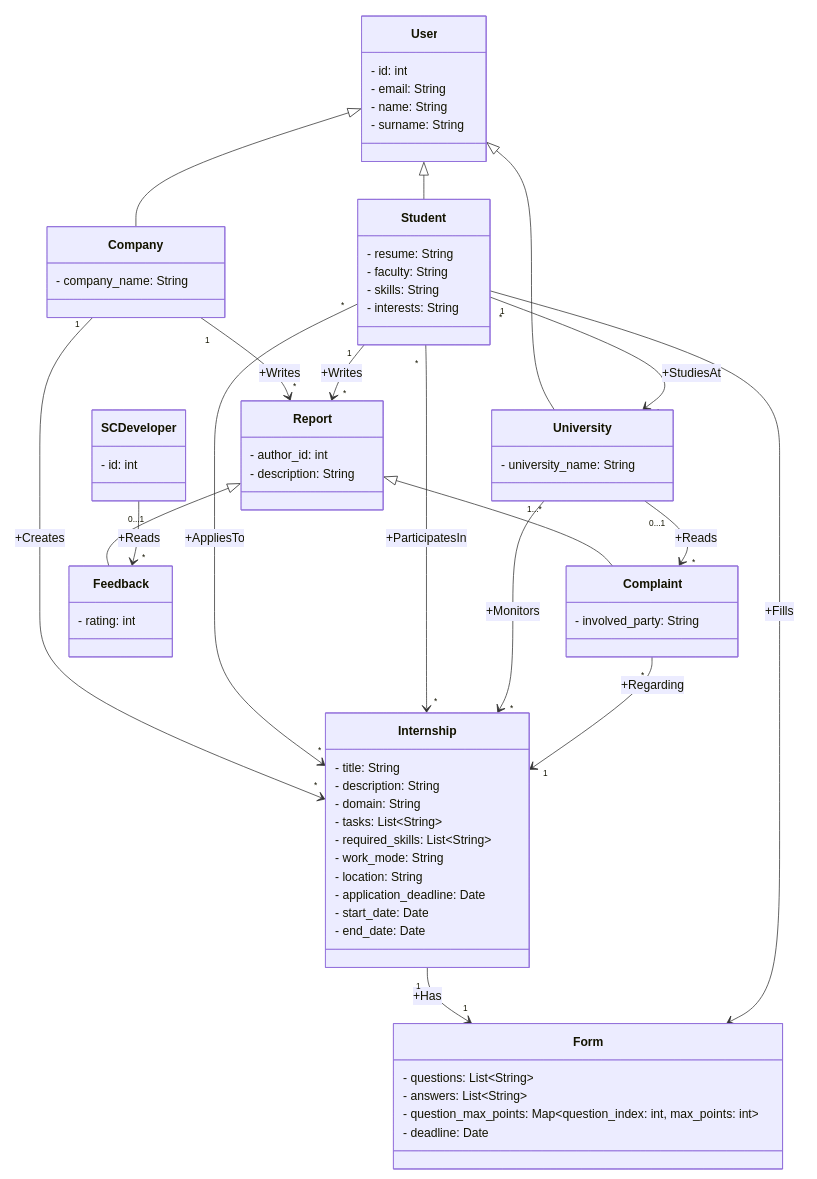
\includegraphics[width=\textwidth]{Images/Class_Diagram}
\end{figure}
\newpage
		\subsubsection{State Chart}
		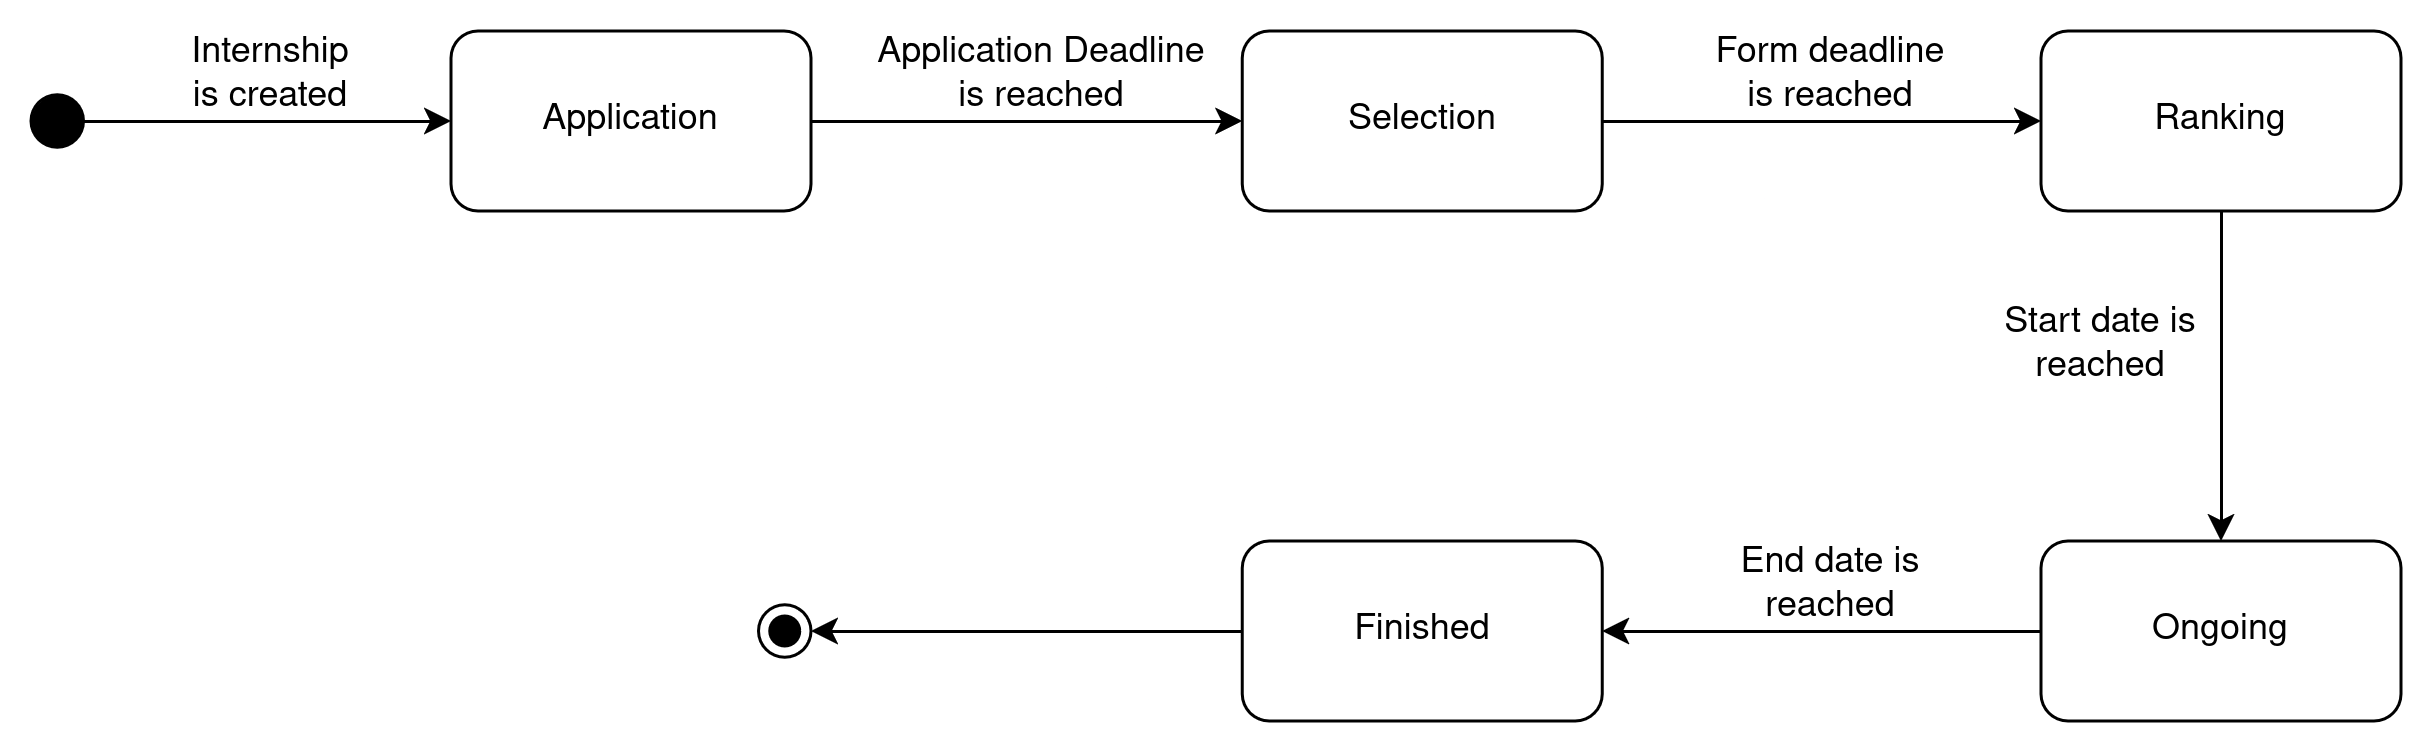
\includegraphics[scale=0.185]{Images/Internship_state_diagram} \\
Right after an internship is created its state is the \textit{Open for applications} state, where students can apply for it. Subsequently to the application deadline, the company will have to select the candidates that suit them the most from those who applied, this is during the \textit{First screening} state. Each selected candidate will receive a notification regarding the result of his application which also includes a form to be filled by a specific date (if they were accepted). Following that date, we arrive at the \textit{Second screening} state where the company has to evaluate the forms filled by each accepted candidate leading to a total score, which S\&C will use to rank all of the candidates. S\&C will then choose (possibly among the best scoring) a subset of those students, all candidates will receive a notification with the result and for those that have been chosen it will also contain a link to a third-party online meeting platform and the date of the interview. After the aforementioned date, we reach the \textit{Ranking} state where the remaining candidates will be further evaluated according to their performance during the interview. This will result in a conclusive ranking which will be used to decide the students that will be accepeted for the internship. Finally, we have the \textit{Ongoing} and \textit{Finished} states that are indicating when the internship is effectively in progress (here both parties can submit complaints) and when it is complete; after which feedback will be asked from students in case they received the offer through the recommendation system. At this point, the internship will be archived as a past project of the company.

	\subsection{Product functions}
\begin{itemize}
\item \textbf{Sign-up and login} \\
Both of these functionalities are going to be available to all user categories. \\
The sign-up functionality allows users to create a verified account to use on the platform. Each user will be asked to provide personal data such as name, surname, email, username and password. The user category will be recognized based on the domain of the email used for the sin-up. \\
The login functionality allows user to gain access to an already existing account using the credentials used during sign-up.
\item \textbf{Update account information} \\
This functionality is only available for all user categories. \\
A student can only update a new CV and change its interests, since all the personal information are extracted from the institutional email. \\
A company can only update the description and add old projects.
\item \textbf{Post internship} \\
This functionality is available only for companies. It allows them to create a new post based on an internship they designed. The post must contain a title, a description describing the various activities, the skills required from the candidates to have a chance in being chosen. It also needs all the deadlines like the applications deadline, after which students are not allow to apply for the internship, and the form compilation deadline, that can be added after the applications deadline. And lastly it needs to specify the location an the period of the internship.
\item \textbf{Create a custom form} \\
This functionality is available only for companies. At some point companies need to create a form that allows the to select faster the candidates for the internship. The form is created by adding a list of questions and for each question it needs to be specified a maximum score that will be used to generate the ranking during the selection process. The form can be created at any time, during the posting process or even before the screening.
\item \textbf{Search for specific internships} \\
This functionality is available for all user categories, but is designed to be used mostly by students. Through a search bar users can look for specific internships or use keywords to filter through the one they are seeking.
\item \textbf{Apply for internship} \\
This functionality is only available for students. This action is going to save the student as a candidate for the internship. At the end of the applications deadline, his CV will be sent to the company with to ones of all the other students that applied for the same internship.
\item \textbf{Screen candidates} \\
This functionality is only available for companies. When the applications period ends and the company is sent the list of candidates, the company's employee will be able to select the candidates that he considers suitable for the internship and discard the one that are not.
\item \textbf{Evaluate form} \\
This functionality is only available for companies. When the company receives a submitted form, this functionality allows them to check the answers given by the candidate and grade them. Once all the answers has been graded and the company's employee closes the form, the system evaluates the total score and adds it to the ranking.
\item \textbf{Send feedback} \\
This functionality is only available for all user categories. Using this feature user can share their opinion with S\&C developers regarding the functionalites implemented in the software.
\end{itemize}

	\subsection{User characteristics}
In this section it is provided a more distinct characterization of the two user categories of the platform.
		\subsubsection{Company}
A company is a representative of a company that wants to advertise its internships. After creating an account as a company, the user gains access to all the company reserved functionality such as internship posting, custom form creation, candidates screening and form evaluation.
		\subsubsection{Student}
A student is an individual whose aim is to either improve his skills or make experience in a professional context. To be able to create an account he must be affiliated with a university and own an institutional email.
		\subsubsection{University}
A university is an institution whose aim, in the context of S\&C application, is to monitor the current status of an internship that involves its students and they are responsible for handling complaints, especially the ones that might require the interruption of the internship.

	\subsection{Assumptions, dependencies and constraints}
\begin{spacing}{1.5}
\textbf{\textit{A1}} - All users have a valid active email. \\
\textbf{\textit{A2}} - Students upload the correct file in the CV section of their account. \\
\textbf{\textit{A3}} - Companies post correct information about existing internships. \\
\textbf{\textit{A4}} - Companies create reasonable forms before the applications deadline. \\
\textbf{\textit{A5}} - The recommendation system is reliable enough. \\
\textbf{\textit{A6}} - Companies check all submitted forms and for each of them grade all questions. \\
\textbf{\textit{A7}} - Feedback and complaints provided by users are truthful and accurate. \\
\textbf{\textit{A8}} - The platform has a list of all the affiliated universities.
\end{spacing}
\newpage
\section{Specific requirements}
	\subsection{External interface requirements}
		\subsubsection{User interfaces}
The platform is presented as a series of different pages, each specialized for one or more features with the same scope. The following ones are considered the most important:
\begin{itemize}
\item \textbf{Login / Sign up page} \\
This page allows the user to choose between one of the two functionalities and insert personal data in different ways based on the option chosen.
\item \textbf{Home Page} \\
In this page users can visualize all the internships that have per posted. In addition there is a search bar that, by entering keywords, allows user to look for specific types of internships.
\item \textbf{Internship creation page} \\
This page is available only for companies, and allow them to fill in all the details required to post about an internship.
\item \textbf{Form design page} \\
This page is available only for companies and it allows them to create custom forms needed to select the candidates that apply for their internship. To create forms, companies write a list of questions and mark them with a maximum score achievable by each one of them. At the end of this process the form can be saved for later use.
\item \textbf{Profile page} \\
This page displays all personal information regarding the user logged in the application. It also allows the user to update different information based on the fact that they are students or companies.
\end{itemize}
		\subsubsection{Hardware interfaces}
The application does not need to provide any kind of hardware interface since it's main purpose is advertising internships and establish a connection between students and companies.
		\subsubsection{Software interfaces}
The software will need to use some external interface to guarantee its correct behavior. For example, to guaranteed the validity of an institutional email, it needs the university to confirm the address, and the same goes for the company.
		\subsubsection{Communication interfaces}
The platform exploits the internet connection to communicate with the main server in order to store and retrieve all the necessary information and also to perform automatic actions such as sending notification, identifying compatible students for the recommendation system and closing an internship's application's process according to the specified deadline.
\newpage
	\subsection{Functional requirements}
		\subsubsection{Functional requirements}
\begin{itemize}
\item \textbf{Account management}
\begin{itemize}
\item[RA1:] The platform shall allow users to register.
\item[RA2:] The platform shall allow users to login using their credentials.
\item[RA3:] The platform shall allow users to update their existing account.
\end{itemize}
\item \textbf{Internships}
\begin{itemize}
\item[RI1:] The platform must allow companies to create internships.
\item[RI2:] The platform must allow students to view all available internships\footnote{Available internships are internships created by companies and that are in the application state; so their application deadline has not arrived yet allowing students to apply to them.}.
\item[RI3:] The platform must allow students to search between the available internships.
\item[RI4:] The platform must allow students to apply for any of the available internships.
\item[RI5:] The platfrom must allow students/companies involved in an internship to complain about the other party.
\end{itemize}
\item \textbf{Notifications}
\begin{itemize}
\item[RN1:] The platform shall notify students when an internship suitable for them has been posted.
\item[RN2:] The platform shall notify students of the result of the first screening.
\item[RN3:] The platform shall notify students of the result of the second screening.
\item[RN4:] The platform shall notify students of the final result of the application.
\item[RN5:] The platform shall notify students/companies to fill a feedback form after the end of the internship.
\item[RN6:] The platform shall notify universities whenever a complaint is filed involving one of their students.
\item[RN7:] The platform shall send companies the list of candidates at the end of the application deadline.
\end{itemize}
\item \textbf{Forms}
\begin{itemize}
\item[RF1:] The platform shall allow companies to create custom forms.
\item[RF2:] The platform shall allow companies to save created forms for later use in an internship selection process.
\item[RF3:] The platform shall allow companies to send the candidates that passed the first screening the form for the second screening.
\item[RF4:] The platform shall allow students to fill and submit the application form.
\item[RF5:] The platform shall allow companies to evaluate a submitted form by grading each question.
\end{itemize}
\item \textbf{Report}
\begin{itemize}
\item[RR1:] The platform shall allow student and companies to write a feedback at the end of an internship.
\item[RR2:] The platform shall allow students and companies involved in an internship to write complaints regarding the other party.
\item[RR3:] The platform shall allow universities to read all complaints that involve their students.
\end{itemize}
\end{itemize}
		\subsubsection{Requirements mapping}
\begin{itemize}
\item[\textbf{[G1]}] - Student can create an account
\begin{table}[H]
\begin{tabular}{| p{0.47\textwidth} | p{0.47\textwidth} |}
\hline
\textbf{Requirements} & \textbf{Assumptions} \\
\hline
\textbf{[RA1]} - The platform shall allow users  to register.
& \textbf{[A1]} - All users have a valid email. \newline 
\textbf{[A8]} - The platform has a list of all affiliated universities. \\
\hline
\end{tabular}
\end{table}

\item[\textbf{[G2]}] - Company can create an account
\begin{table}[H]
\begin{tabular}{| p{0.47\textwidth} | p{0.47\textwidth} |}
\hline
\textbf{Requirements} & \textbf{Assumptions} \\
\hline
\textbf{[RA1]} - The platform shall allow users  to register.
& \textbf{[A1]} - All users have a valid email. \\
\hline
\end{tabular}
\end{table}

\item[\textbf{[G3]}] - Users can update their accounts
\begin{table}[H]
\begin{tabular}{| p{0.47\textwidth} | p{0.47\textwidth} |}
\hline
\textbf{Requirements} & \textbf{Assumptions} \\
\hline
\textbf{[RA3]} - The platform shall allow users to update their existing account.
& \textbf{[A2]} - Students upload the correct file in the CV section of the account. \\
\hline
\end{tabular}
\end{table}

\item[\textbf{[G4]}] - Companies can create internships
\begin{table}[H]
\begin{tabular}{| p{0.47\textwidth} | p{0.47\textwidth} |}
\hline
\textbf{Requirements} & \textbf{Assumptions} \\
\hline
\textbf{[RI1]} - The platform must allow companies to create internships.
& \textbf{[A3]} - Companies post correct information about existing internships. \\
\hline
\end{tabular}
\end{table}

\item[\textbf{[G5]}] - Students can view all available internships
\begin{table}[H]
\begin{tabular}{| p{0.47\textwidth} | p{0.47\textwidth} |}
\hline
\textbf{Requirements} & \textbf{Assumptions} \\
\hline
\textbf{[RI2]} - The platform must allow students to view all available internships. \newline
\textbf{[RI3]} - The platform must allow students to search between the available internships.
& None. \\
\hline
\end{tabular}
\end{table}

\item[\textbf{[G6]}] - Companies can create forms for students to fill
\begin{table}[H]
\begin{tabular}{| p{0.47\textwidth} | p{0.47\textwidth} |}
\hline
\textbf{Requirements} & \textbf{Assumptions} \\
\hline
\textbf{[RF1]} - The platform shall allow companies to create custom forms. \newline
\textbf{[RF2]} - The platform shall allow companies to save created forms for later use in an internship selection process.
& \textbf{[A4]} - Companies create reasonable forms before the applications deadline. \\
\hline
\end{tabular}
\end{table}

\item[\textbf{[G7]}] - Recommendation system
\begin{table}[H]
\begin{tabular}{| p{0.47\textwidth} | p{0.47\textwidth} |}
\hline
\textbf{Requirements} & \textbf{Assumptions} \\
\hline
\textbf{[RN1]} - The platform shall notify students when an internship suitable for them has been posted.
& \textbf{[A5]} - The recommendation system is reliable enough. \\
\hline
\end{tabular}
\end{table}

\item[\textbf{[G8]}] - Students can apply for the internships
\begin{table}[H]
\begin{tabular}{| p{0.47\textwidth} | p{0.47\textwidth} |}
\hline
\textbf{Requirements} & \textbf{Assumptions} \\
\hline
\textbf{[RI4]} - The platform must allow students to apply for any available internship.
& None. \\
\hline
\end{tabular}
\end{table}

\item[\textbf{[G9]}] - Form evaluation
\begin{table}[H]
\begin{tabular}{| p{0.47\textwidth} | p{0.47\textwidth} |}
\hline
\textbf{Requirements} & \textbf{Assumptions} \\
\hline
\textbf{[RN7]} - The platform shall send companies the list of candidates st the end of the application deadline. \newline
\textbf{[RF3]} - The platform shall allow companies to send the candidates that passed the first screening the form for the second screening. \newline
\textbf{[RF4]} - The platform shall allow students to fill and submit the application form. \newline
\textbf{[RF5]} - The platform shall allow companies to evaluate a submitted form by grading each question.
& \textbf{[A6]} - Companies check all submitted forms and for each of them grade all questions. \\
\hline
\end{tabular}
\end{table}

\item[\textbf{[G10]}] - Ranking candidates
\begin{table}[H]
\begin{tabular}{| p{0.47\textwidth} | p{0.47\textwidth} |}
\hline
\textbf{Requirements} & \textbf{Assumptions} \\
\hline
\textbf{[RN2]} - The platform shall notify students of the result of the first screening. \newline
\textbf{[RN3]} - The platform shall notify students of the result of the second screening. \newline
\textbf{[RN4]} - The platform shall notify students of the final result of the application.
& \textbf{[A6]} - Companies check all submitted forms and for each of them grade all questions. \\
\hline
\end{tabular}
\end{table}

\item[\textbf{[G11]}] - Users can provide feedbacks
\begin{table}[H]
\begin{tabular}{| p{0.47\textwidth} | p{0.47\textwidth} |}
\hline
\textbf{Requirements} & \textbf{Assumptions} \\
\hline
\textbf{[RN5]} - The platform shall notify students/companies to fill a feedback form after the end of the internship. \newline
\textbf{[RR1]} - The platform shall allow students and companies to write a feedback at the end of an internship.
& \textbf{[A7]} - Feedback and complaints provided by users are truthful and accurate. \\
\hline
\end{tabular}
\end{table}

\newpage
\item[\textbf{[G12]}] - Complaints management
\begin{table}[H]
\begin{tabular}{| p{0.47\textwidth} | p{0.47\textwidth} |}
\hline
\textbf{Requirements} & \textbf{Assumptions} \\
\hline
\textbf{[RI5]} - The platform must allow students/companies involved in an internship to complain about the other party. \newline
\textbf{[RN6]} - The platform shall notify universities whenever a complaint is filed involving one of their students. \newline
\textbf{[RR2]} - The platform shall allow students and companies involved in an internship to write complaints regarding the other party. \newline
\textbf{[RR3]} - The platform shall allow universities to read all complaints that involve their students.
& \textbf{[A7]} - Feedback and complaints provided by users are truthful and accurate. \\
\hline
\end{tabular}
\end{table}
\end{itemize}

		\subsubsection{Use cases and diagrams}
In this section are reported some of the most notable use cases for the S\&C application. \\
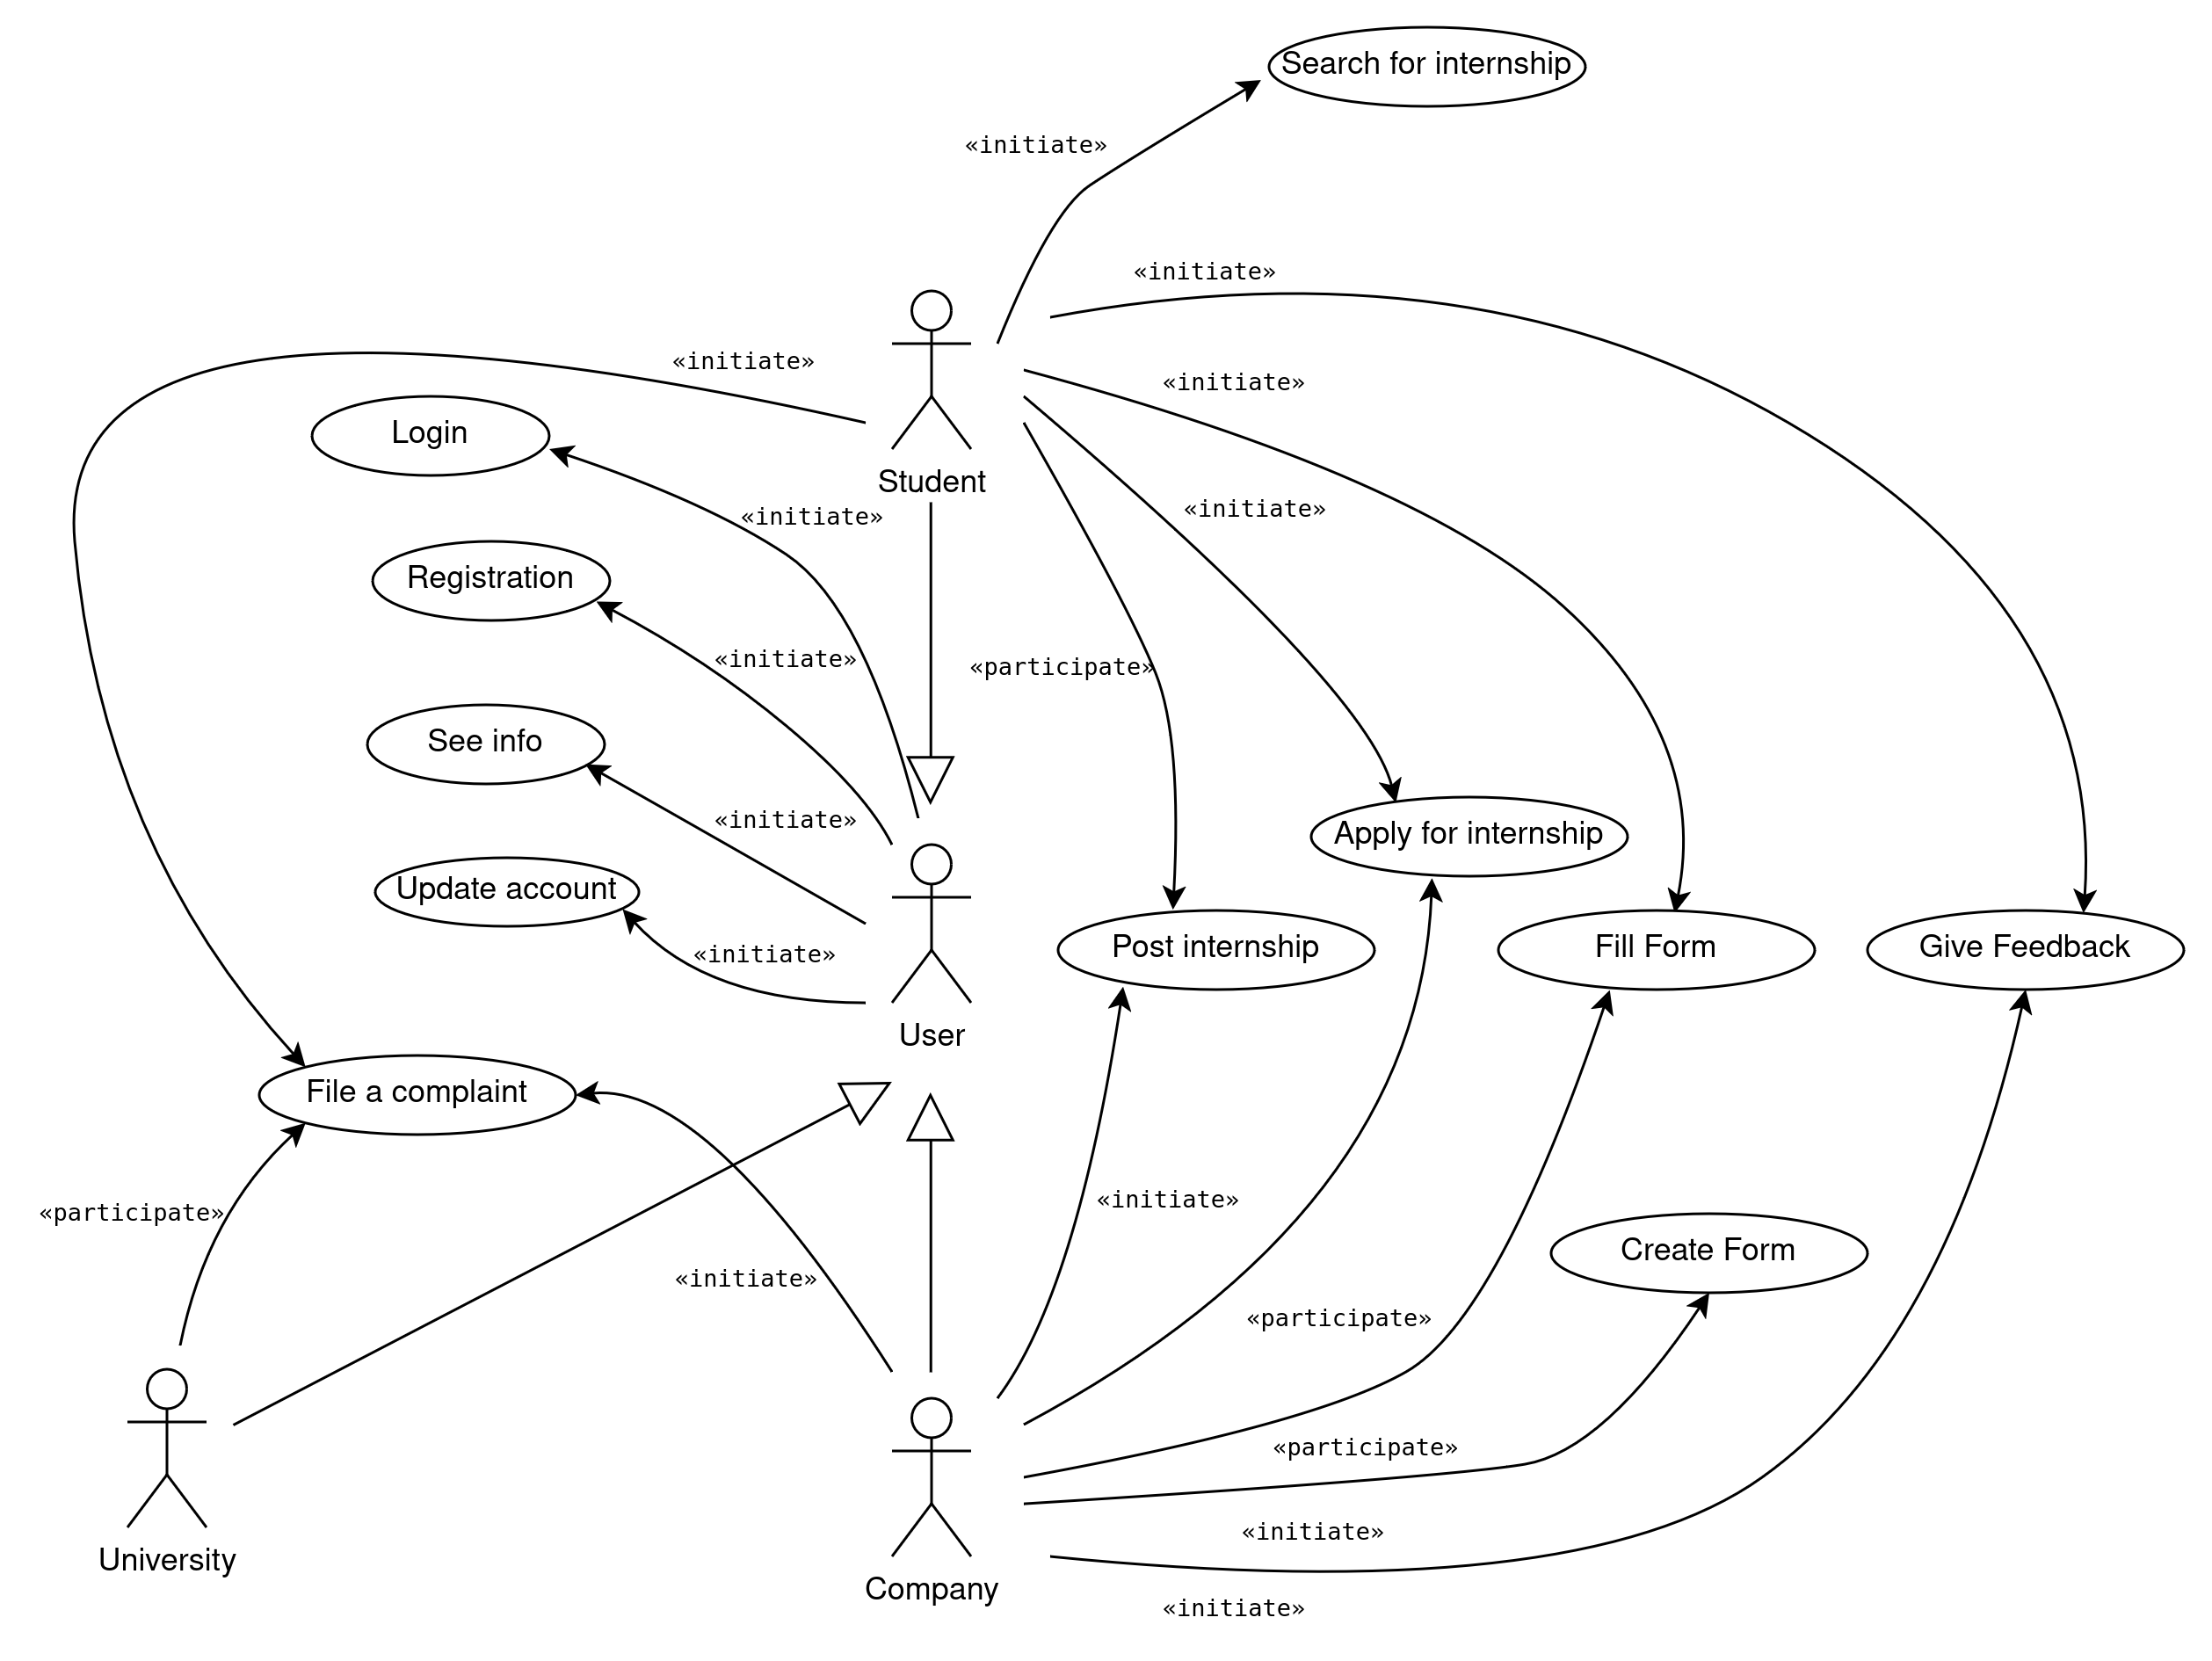
\includegraphics[width=\textwidth]{Images/Use_case_diagram}
\newpage
\large{\textbf{[UC1]}}
\begin{table}[H]
\begin{tabular}{| p{0.3\textwidth} | p{0.64\textwidth} |}
\hline
\textbf{Name}
& Register user \\
\hline
\textbf{Actors}
& User \\
\hline
\textbf{Entry conditions}
& User opens the platform without an account \\
\hline
\textbf{Events flow}
& 1. The user starts the registration process \newline
2. The system asks the user to choose if he/she is a student or a company and to provide: name, surname, username, email and password \newline
3. User fills in the text fields with the required information \newline
4. The system checks if email or username have been already used by another user to register \newline
5. System updates the database with the user’s information and 
displays a message of confirmed registration  \\
\hline
\textbf{Exit conditions}
& User successfully registers on the platform \\
\hline
\textbf{Exceptions}
& The user enters invalid credentials, such as non existent or already registered email \\
\hline
\end{tabular}
\end{table}

\begin{center}
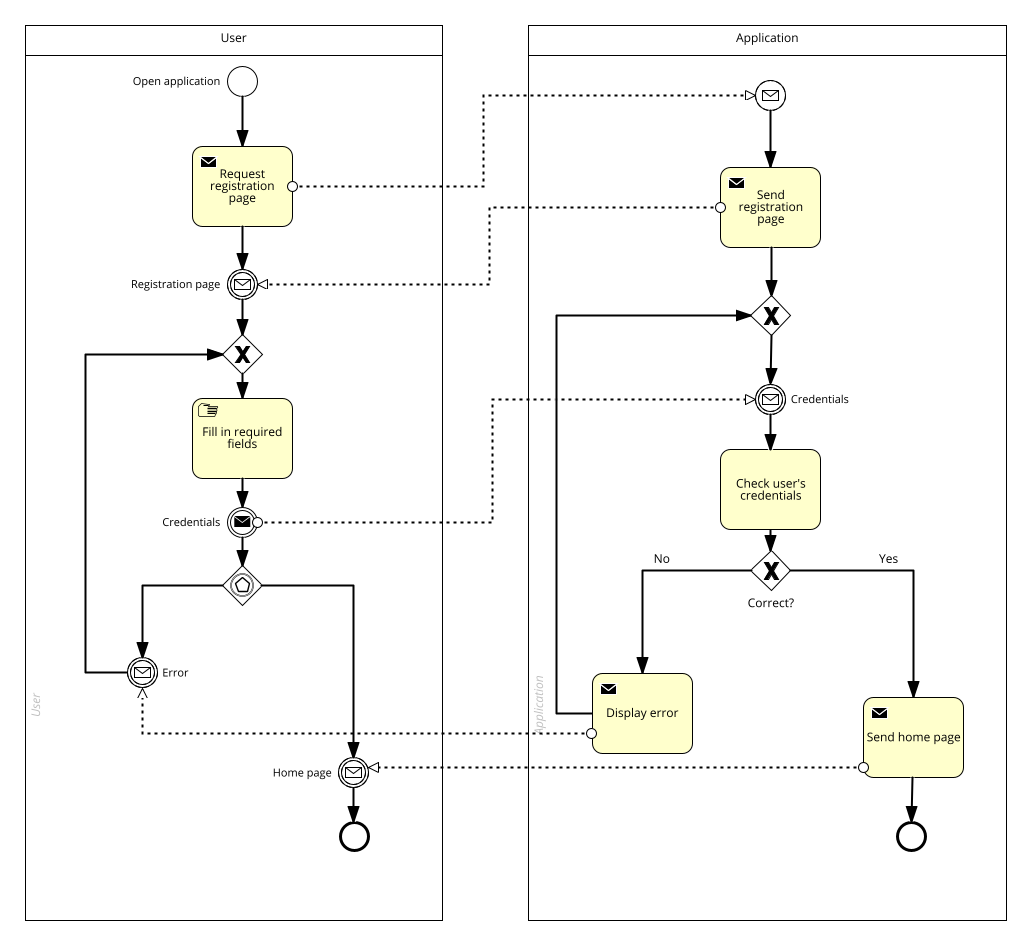
\includegraphics[width=\textwidth]{Images/UC1}
\end{center}

\newpage

\large{\textbf{[UC2]}}
\begin{table}[H]
\begin{tabular}{| p{0.3\textwidth} | p{0.64\textwidth} |}
\hline
\textbf{Name}
& User login \\
\hline
\textbf{Actors}
& User \\
\hline
\textbf{Entry conditions}
& User opens the platform while having a registered account \\
\hline
\textbf{Events flow}
& 1. User inserts fills in the appropriate fields for the login with his credentials (username and password) and presses the “Login” button \newline
2. The system checks if the information inserted are correct \newline
3. The system displays the home page to the user \\
\hline
\textbf{Exit conditions}
& The user is logged in the platform \\
\hline
\textbf{Exceptions}
& When the user inserts the wrong combination of username and password and presses the "Login" button, the application displays an error message. \\
\hline
\end{tabular}
\end{table}

\begin{center}
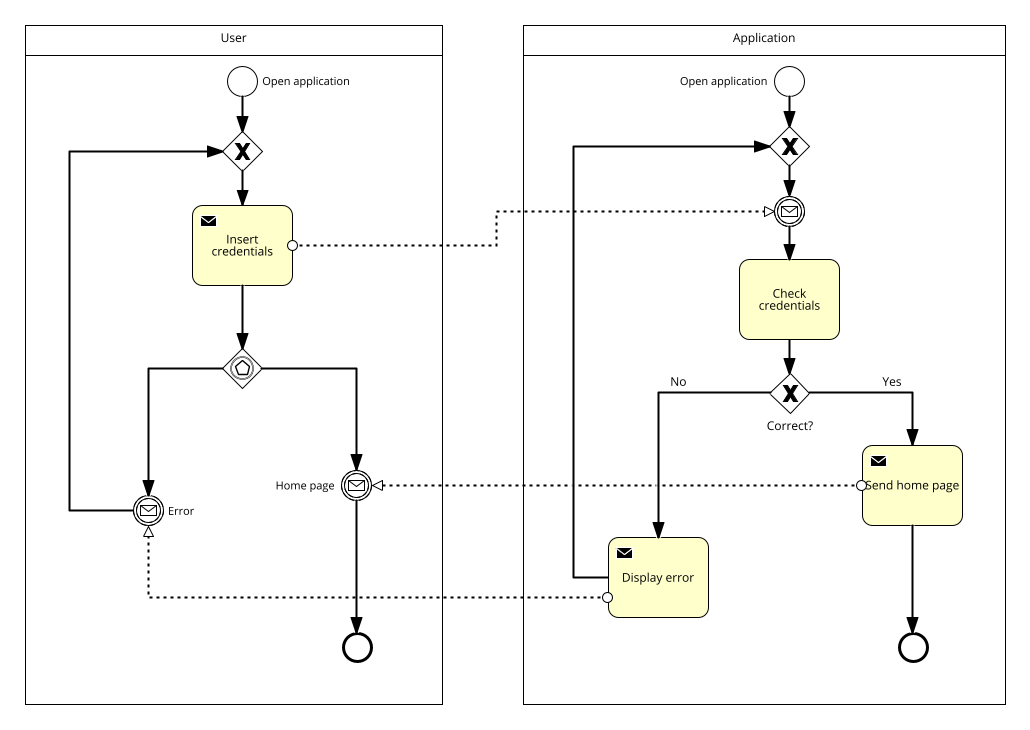
\includegraphics[width=\textwidth]{Images/UC2}
\end{center}

\newpage

\large{\textbf{[UC3]}}
\begin{table}[H]
\begin{tabular}{| p{0.3\textwidth} | p{0.64\textwidth} |}
\hline
\textbf{Name}
& Internship creation \\
\hline
\textbf{Actors}
& Company ; \textit{Student (Notified)} \\
\hline
\textbf{Entry conditions}
& User is logged in a company account \\
\hline
\textbf{Events flow}
& 1. Company requests to create an internship post \newline
2. The system asks the company all the required information to create the post \newline
3. The company submits the requested information \newline
4. The system validates the information provided by the company \newline
5. The system adds the internship to its database and and notifies all compatible student \\
\hline
\textbf{Exit conditions}
& The company successfully created an internship and the compatible students received a notification from the system \\
\hline
\textbf{Exceptions}
& When attempting to create the post if the company doesn't insert all the required information, the application displays an error message \\
\hline
\end{tabular}
\end{table}

\begin{center}
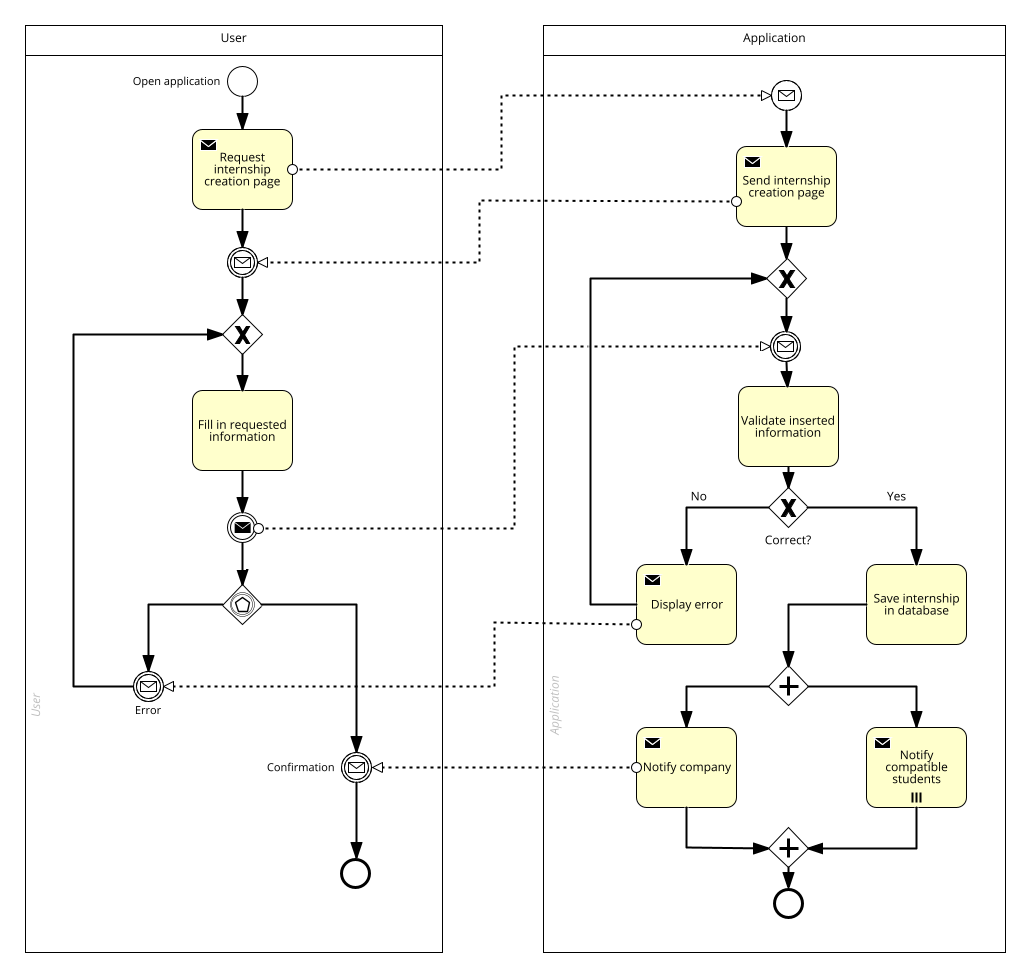
\includegraphics[width=0.95\textwidth]{Images/UC3}
\end{center}

\newpage

\large{\textbf{[UC4]}}
\begin{table}[H]
\begin{tabular}{| p{0.3\textwidth} | p{0.64\textwidth} |}
\hline
\textbf{Name}
& Student proactive search \\
\hline
\textbf{Actors}
& Student \\
\hline
\textbf{Entry conditions}
& - User is logged in with a student account \\
\hline
\textbf{Events flow}
& 1. The student insert some keywords in the search bar in the home page \newline
2. The system filters the internships that satisfy the keywords \newline
3. The student chooses an internship and applies for it \\
\hline
\textbf{Exit conditions}
& The student successfully applies for an internship \\
\hline
\textbf{Exceptions}
& If there are no suitable internships the system returns a warning message \\
\hline
\end{tabular}
\end{table}

\begin{center}
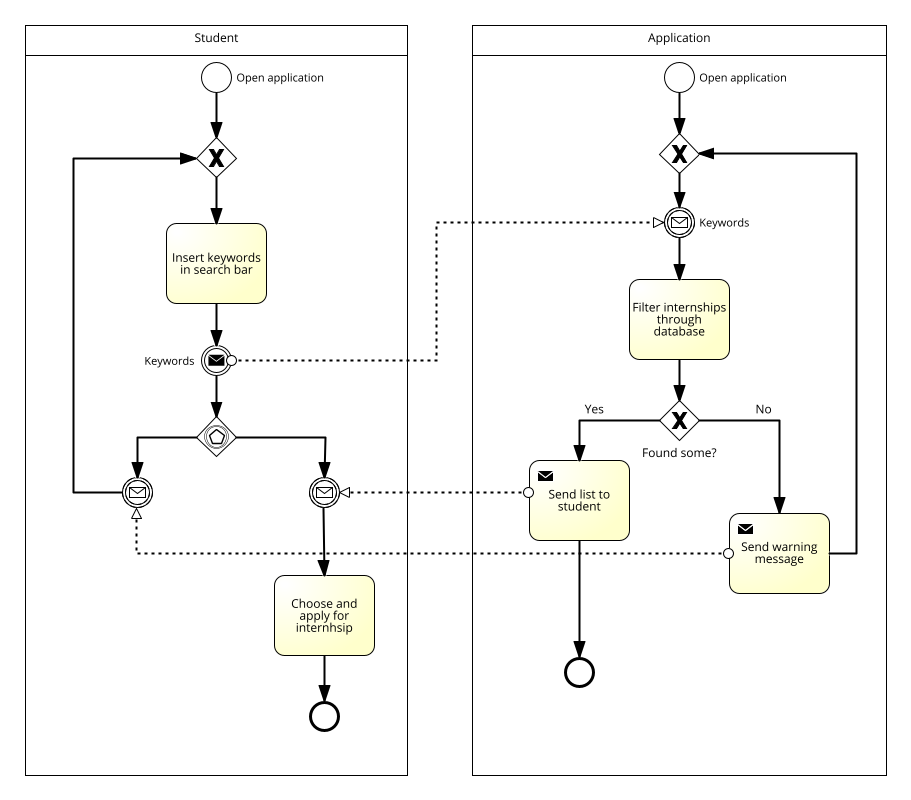
\includegraphics[width=\textwidth]{Images/UC4}
\end{center}

\newpage

\large{\textbf{[UC5]}}
\begin{table}[H]
\begin{tabular}{| p{0.3\textwidth} | p{0.64\textwidth} |}
\hline
\textbf{Name}
& Selection process (part 1) \\
\hline
\textbf{Actors}
& Company ; Student \\
\hline
\textbf{Entry conditions}
& A student has applied for an internship \\
\hline
\textbf{Events flow}
& 1. Student applies for an internship \newline
2. When the application deadline is reached, the company receives the list of all the candidates \newline
3. The company performs a first screening and sends to the remaining ones a form to fill in \\
\hline
\textbf{Exit conditions}
& The student is selected during the first screening or rejected \\
\hline
\textbf{Exceptions}
& None \\
\hline
\end{tabular}
\end{table}

\begin{center}
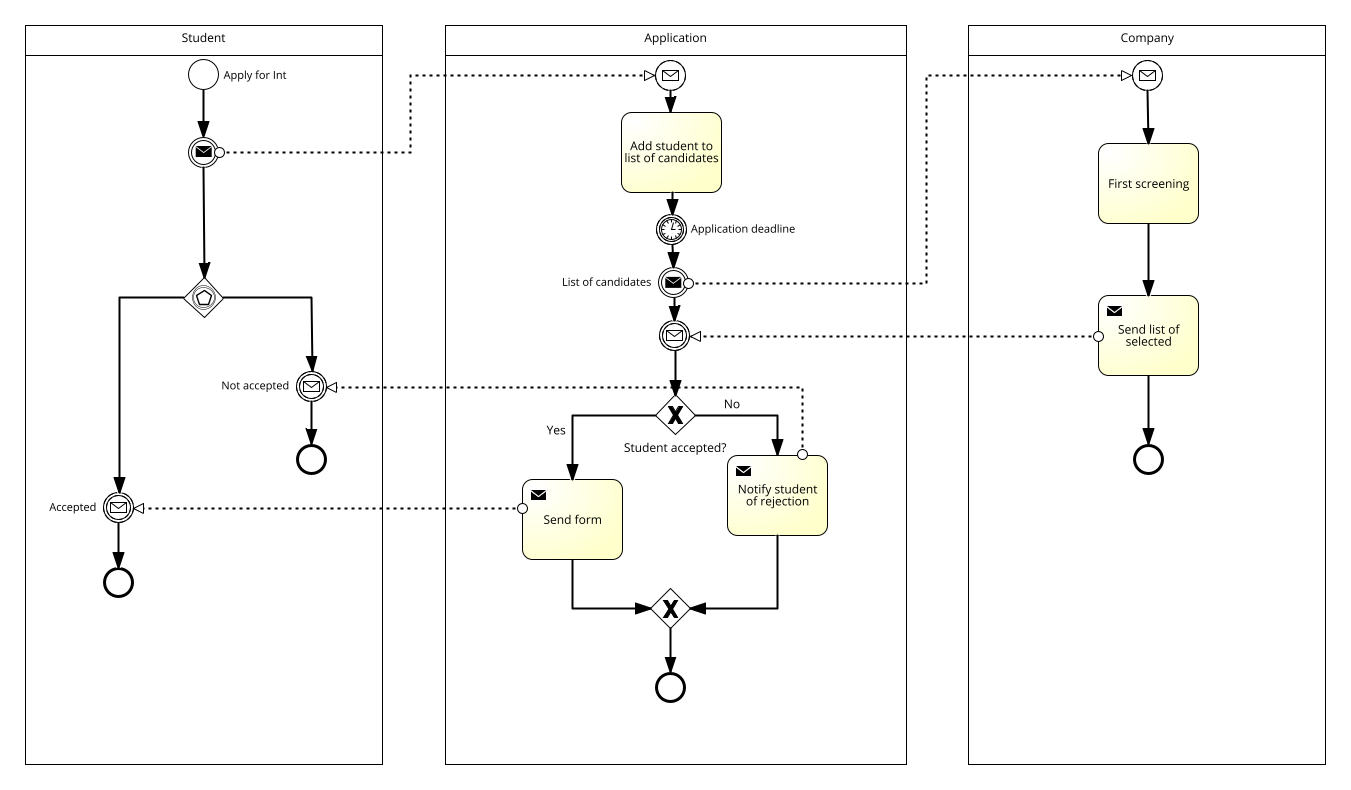
\includegraphics[width=\textwidth]{Images/UC5}
\end{center}

\newpage

\large{\textbf{[UC6]}}
\begin{table}[H]
\begin{tabular}{| p{0.3\textwidth} | p{0.64\textwidth} |}
\hline
\textbf{Name}
& Selection process (part 2) \\
\hline
\textbf{Actors}
& Company ; Student \\
\hline
\textbf{Entry conditions}
& The student applied for an internship \newline
The student has been selected during the first screening \\
\hline
\textbf{Events flow}
& 1. After receiving the form, the student fills it and submits it \newline
2. After the form deadline, the company evaluates all forms and submits the scores \newline
3. The system creates a ranking and sends it to the company \newline
4. The company submits the list of accepted candidates \newline
5. The candidates are notified of the second screening's outcome \\
\hline
\textbf{Exit conditions}
& The student is either selected or rejected during the second screening \\
\hline
\textbf{Exceptions}
& None \\
\hline
\end{tabular}
\end{table}

\begin{center}
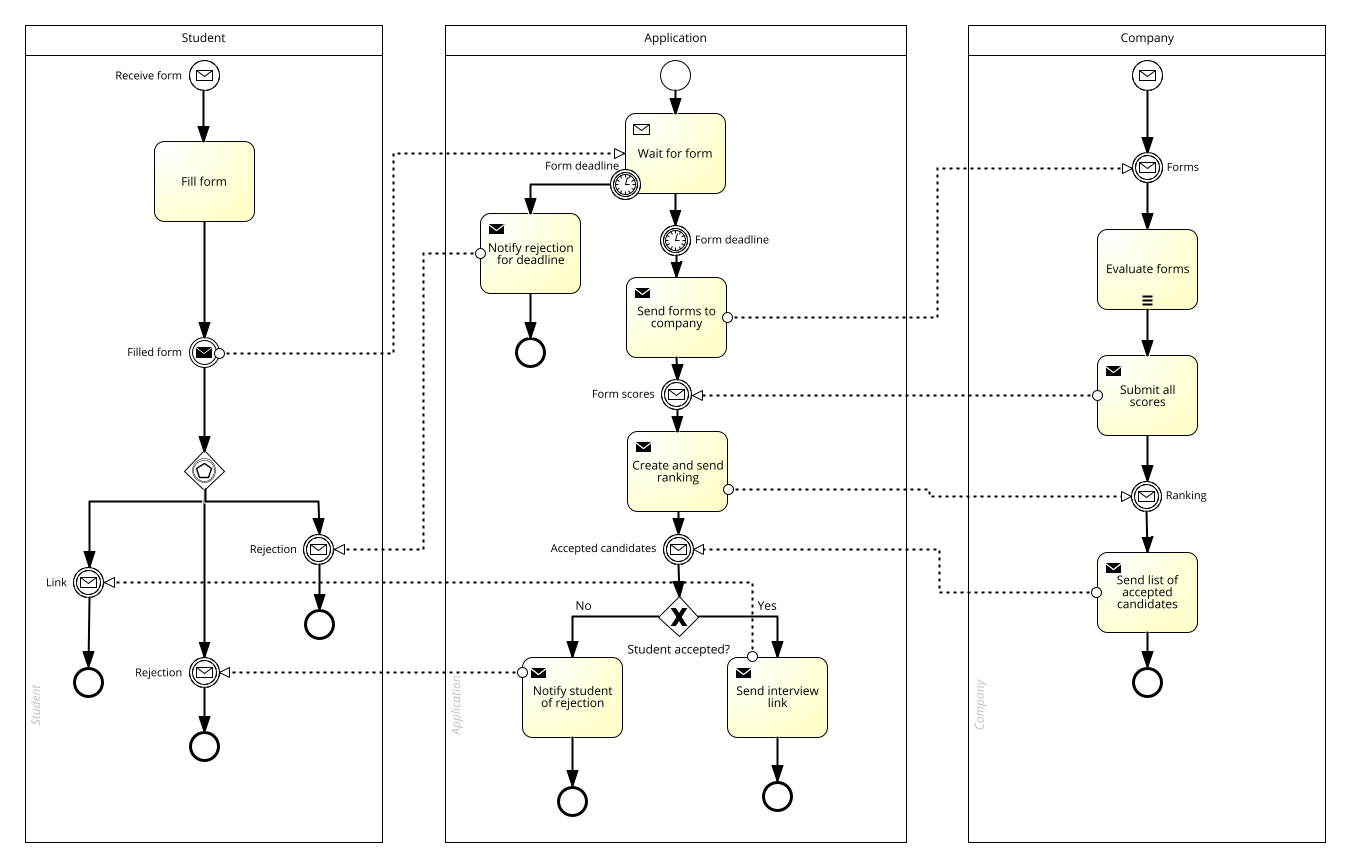
\includegraphics[width=\textwidth]{Images/UC6}
\end{center}

\newpage

\large{\textbf{[UC7]}}
\begin{table}[H]
\begin{tabular}{| p{0.3\textwidth} | p{0.64\textwidth} |}
\hline
\textbf{Name}
& Selection process (part 3) \\
\hline
\textbf{Actors}
& Company ; Student \\
\hline
\textbf{Entry conditions}
& The student applied for an internship \newline
The company received the updated ranking \\
\hline
\textbf{Events flow}
& 1. The company picks the top n candidates and sends the a link for the interview \newline
2. After the interviews, the ranking is updated and the top candidates are accepted for the internship \newline
3. The accepted candidates receive a notification with all the information needed for the internship \\
\hline
\textbf{Exit conditions}
& The student has been either rejected or accepted \\
\hline
\textbf{Exceptions}
& None \\
\hline
\end{tabular}
\end{table}

\begin{center}
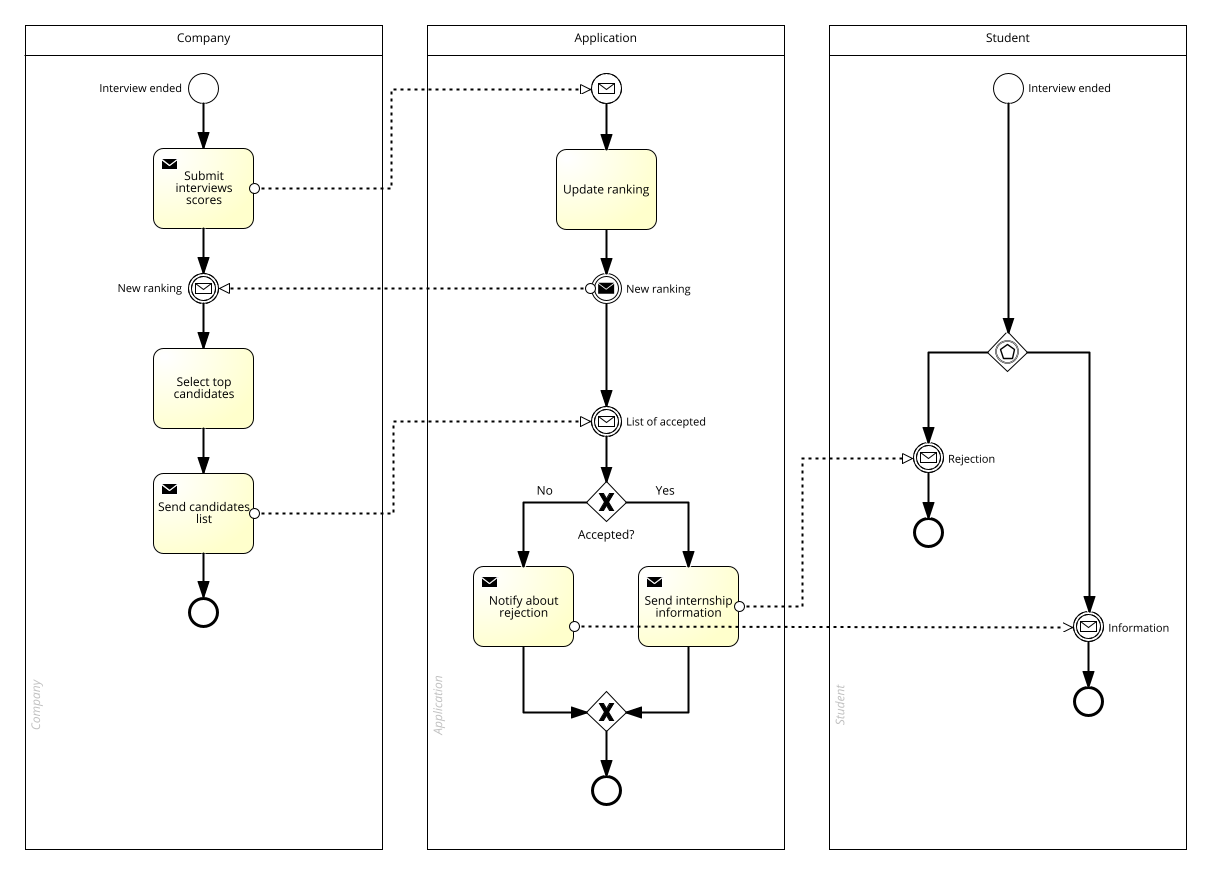
\includegraphics[width=\textwidth]{Images/UC7}
\end{center}

\newpage

\large{\textbf{[UC8]}}
\begin{table}[H]
\begin{tabular}{| p{0.3\textwidth} | p{0.64\textwidth} |}
\hline
\textbf{Name}
& User complaint \\
\hline
\textbf{Actors}
& User \\
\hline
\textbf{Entry conditions}
& A student is participating in an internship \\
\hline
\textbf{Events flow}
& 1. The user requests for the complaint page \newline
2. The system sends the page back \newline
3. The user writes the complaint and submits it \newline
4. The university is notified of the complaint \\
\hline
\textbf{Exit conditions}
& The complaint is saved in the system databases \\
\hline
\textbf{Exceptions}
& None \\
\hline
\end{tabular}
\end{table}

\begin{center}
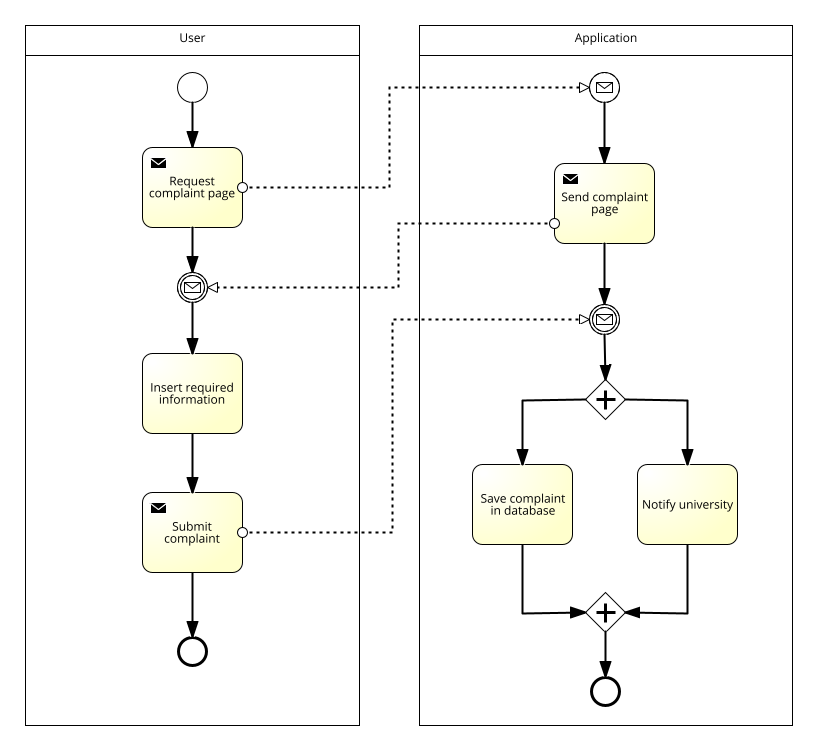
\includegraphics[width=\textwidth]{Images/UC8}
\end{center}

\newpage

\large{\textbf{[UC9]}}
\begin{table}[H]
\begin{tabular}{| p{0.3\textwidth} | p{0.64\textwidth} |}
\hline
\textbf{Name}
& User provides feedback \\
\hline
\textbf{Actors}
& User \\
\hline
\textbf{Entry conditions}
& The internship was concluded \\
\hline
\textbf{Events flow}
& 1. When an internship is concluded, the users involved in the internship receive a notification to remind them to give a feedback \newline
2. The user writes a feedback and submits it \newline
3. The feedback is saved int the system database \\
\hline
\textbf{Exit conditions}
& The feedback is saved in the system databases \\
\hline
\textbf{Exceptions}
& None \\
\hline
\end{tabular}
\end{table}

\begin{center}
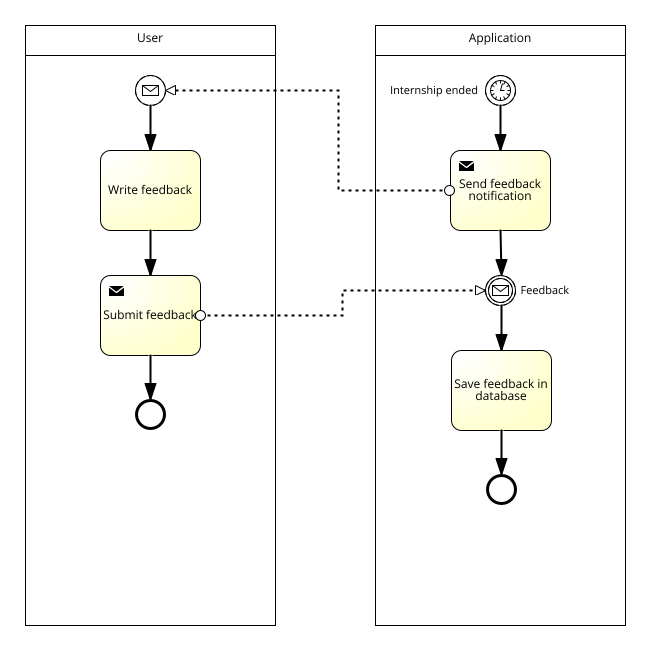
\includegraphics[width=\textwidth]{Images/UC9}
\end{center}

\newpage

\large{\textbf{[UC10]}}
\begin{table}[H]
\begin{tabular}{| p{0.3\textwidth} | p{0.64\textwidth} |}
\hline
\textbf{Name}
& User updates profile \\
\hline
\textbf{Actors}
& User \\
\hline
\textbf{Entry conditions}
& The user is logged in the platform \\
\hline
\textbf{Events flow}
& 1. The user opens its profile page and requests the edit mode \newline
2. The user updates some information and submits it \newline
3. The system checks the information and then saves it in the database \\
\hline
\textbf{Exit conditions}
& The user successfully updates the profile \\
\hline
\textbf{Exceptions}
& The user leaves some required fields empty \\
\hline
\end{tabular}
\end{table}

\begin{center}
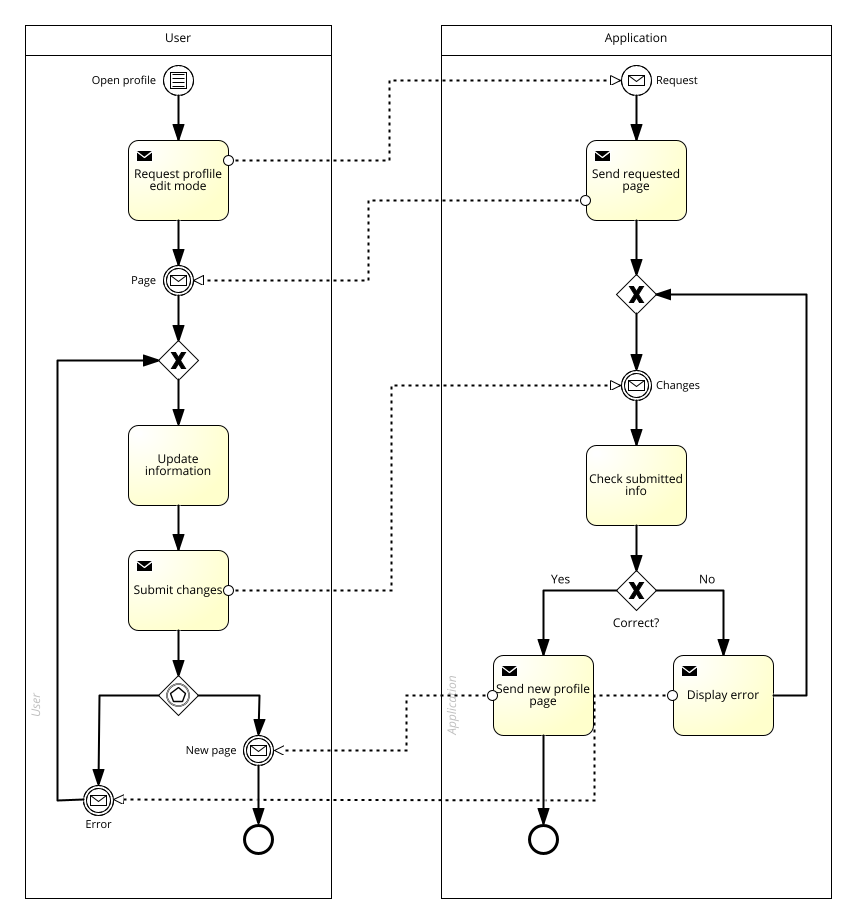
\includegraphics[width=\textwidth]{Images/UC10}
\end{center}

\newpage

\large{\textbf{[UC11]}}
\begin{table}[H]
\begin{tabular}{| p{0.3\textwidth} | p{0.64\textwidth} |}
\hline
\textbf{Name}
& Company creates a form \\
\hline
\textbf{Actors}
& Company \\
\hline
\textbf{Entry conditions}
& The user is logged with a company account \\
\hline
\textbf{Events flow}
& 1. The user requests the form creation page \newline
2. The user creates a list of questions and marks them with a maximum score \newline
3. The user saves the form in the system for later use \newline
4. The system checks the information and then saves it in the database \\
\hline
\textbf{Exit conditions}
& The user successfully creates a form \\
\hline
\textbf{Exceptions}
& The user doesn't mark every question with a max score \\
\hline
\end{tabular}
\end{table}

\begin{center}
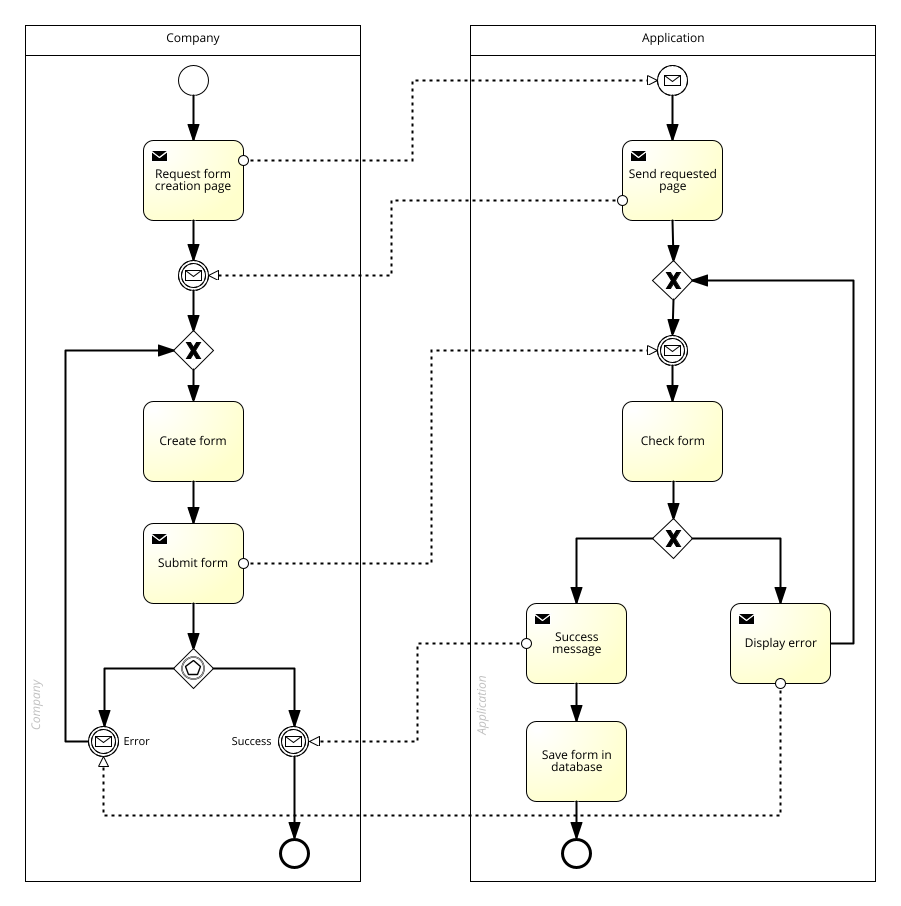
\includegraphics[width=\textwidth]{Images/UC11}
\end{center}

\newpage

\large{\textbf{[UC12]}}
\begin{table}[H]
\begin{tabular}{| p{0.3\textwidth} | p{0.64\textwidth} |}
\hline
\textbf{Name}
& University monitors internship \\
\hline
\textbf{Actors}
& University \\
\hline
\textbf{Entry conditions}
& A complaint is submitted \\
\hline
\textbf{Events flow}
& 1. The university receives a notification regarding a complaint \newline
2. The university opens the application \newline
3. The university reads the complaint \\
\hline
\textbf{Exit conditions}
& The university has read the complaint \\
\hline
\textbf{Exceptions}
& None \\
\hline
\end{tabular}
\end{table}

\begin{center}
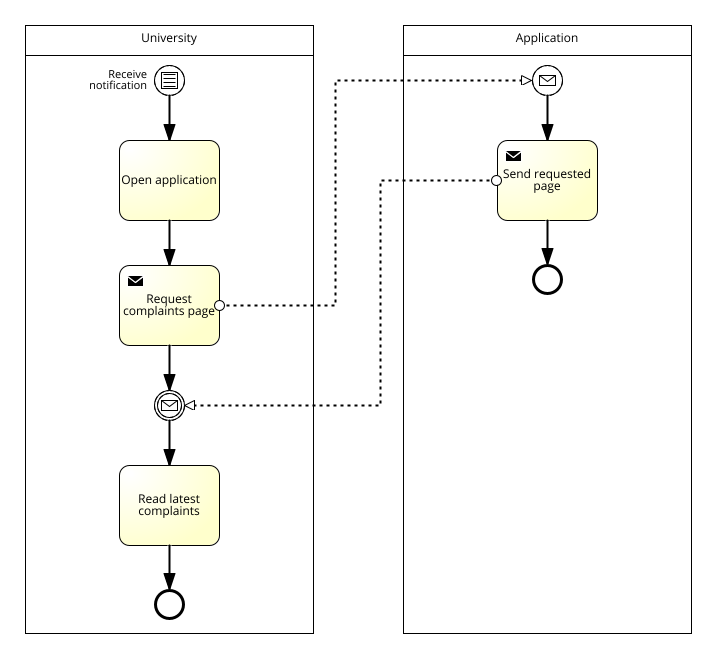
\includegraphics[width=\textwidth]{Images/UC12}
\end{center}

\newpage

		\subsubsection{Traceability matrix}
\begin{table}[H]
\begin{tabular}{| >{\arraybackslash}m{0.64\textwidth} | >{\centering\arraybackslash}m{0.3\textwidth} |}
\hline
\textbf{Requirement} & \textbf{Use case} \\
\hline
RA1 - The platform shall allow users to register. & Register user \\
\hline
RA2 - The platform shall allow users to login using their credentials. & User login \\
\hline
RA3 - The platform shall allow users to update their existing account. & User updates profile \\
\hline
RI1 - The platform must allow companies to create internships. & Internship creation \\
\hline
RI2 - The platform must allow students to view all available internships & Student proactive search \\
\hline
RI3 - The platform must allow students to search between the available internships. & Student proactive search \\
\hline
RI4 - The platform must allow students to apply for any of the available internships. & Student proactive search \\
\hline
RI5 - The platfrom must allow students/companies involved in an internship to complain about the other party. & User complaint \\
\hline
RN1 - The platform shall notify students when an internship suitable for them has been posted. & Internship creation \\
\hline
RN2 - The platform shall notify students of the result of the first screening. & Selection process (part 1) \\
\hline
RN3 - The platform shall notify students of the result of the second screening. & Selection process (part 2) \\
\hline
RN4 - The platform shall notify students of the final result of the application. & Selection process (part 3) \\
\hline
RN5 - The platform shall notify students/companies to fill a feedback form after the end of the internship. & User provides feedback \\
\hline
RN6 - The platform shall notify universities whenever a complaint is filed involving one of their students. & User complaint \\
\hline
RN7 - The platform shall send companies the list of candidates at the end of the application deadline. & Selection process (part 1) \\
\hline
RF1 - The platform shall allow companies to create custom forms. & Company creates a form \\
\hline
RF2 - The platform shall allow companies to save created forms for later use in an internship selection process. & Company creates a form \\
\hline
RF3 - The platform shall allow companies to send the candidates that passed the first screening the form for the second screening. & Selection process (part 1) \\
\hline
RF4 - The platform shall allow students to fill and submit the application form. & Selection process (part 2) \\
\hline
RF5 - The platform shall allow companies to evaluate a submitted form by grading each question. & Selection process (part 2) \\
\hline
RR1 - The platform shall allow student and companies to write a feedback at the end of an internship. & User provides feedback \\
\hline
RR2 - The platform shall allow students and companies involved in an internship to write complaints regarding the other party. & User complaint \\
\hline
RR3 - The platform shall allow universities to read all complaints that involve their students. & University monitors internship \\
\hline
\end{tabular}
\end{table}

\newpage

	\subsection{Performance requirements}
Most of the times the application acts as a database for companies' internships, when students are navigating through the available offers or proactively searching for them. \\
The rest of the time the application acts as a simple notification system that allows students to be alerted when an interesting offer is posted, or to be notified of the result of the various screenings when applied for an internship. \\
For this reason the system's performance limits must be calculated by considering this two conditions: 
\begin{itemize}
\item The minimization of the time needed for querying the database.
\item The minimization of the time needed to send notifications.
\end{itemize}
	
	\subsection{Design constraints}	
		\subsubsection{Standards compliance}
\textbf{Disclosures and privacy policies} \\
The application fully comply with data protection regulations, such as the General Data Protection Regulation (GDPR) for European users and the California Consumer Privacy Act (CCPA) for American users. The system only collects data necessary for its operation, and users have the right to access, modify, or delete their data as per GDPR requirements.
\vspace{1\baselineskip}\\
\textbf{Encryption and anonymizing} \\
Since the application highly depends on internet connectivity for syncing data, user authentication, and notifications, security is a top priority. The software uses TLS 1.2/1.3 encryption to ensures that all data exchanged between users’ devices and the servers is encrypted and protected from interception or unauthorized access.
\vspace{1\baselineskip}\\
\textbf{Data storage} \\
For data storage, the software complies with ISO/IEC 27001 standards, ensuring high levels of security, and data protection. This includes regular data backups, disaster recovery protocols, and server redundancy to prevent data loss and maintain consistent up time.
		
		\subsubsection{Hardware limitations}
The software shall be designed to run efficiently on minimal hardware, making it accessible across a wide range of devices, including older computers and lower-end mobile devices.
		
		\subsubsection{Any other constraints}
The platform is intended to connect student and companies from all over the world. For this reason, it should be designed completely in English, allowing all user to understand all the features.
		
	\subsection{Software system attributes}
		\subsubsection{Reliability}
The application shall be designed to operate reliably under a range of conditions, and the notification system must be robust enough to ensure that users can consistently complete their tasks without any problems, like applying for internships, filling forms and so on.
		
		\subsubsection{Availability}
To maximize availability, the application shall operate a distributed cloud infrastructure with redundant servers, to ensure consistent up time. The application achieves a targeted up time of 99.9\%, minimizing disruptions and providing users with dependable access whenever needed.
		
		\subsubsection{Security}
As mentioned in section 3.4.1, to match the GDPR compliance, user authentication shall be handled via secure protocols, such as OAuth 2.0, allowing users to log in through trusted providers while protecting their credentials. \\
In addition the system use TLS 1.2/1.3 encryption for data transmission, to protect it from external parties.
		
		\subsubsection{Maintainability}
The application is developed using modular code architecture that makes updates and bug fixes as efficient and straightforward as possible. The software code base is well-documented and follows standard coding practices and patterns, making it easy for developers to understand and work with. Additionally, a version control system, such as Git, is in place to manage updates, ensuring that updates do not disrupt user experience.
		
		\subsubsection{Portability}
The software shall be designed to be portable across multiple platforms, including Windows, macOS, Linux, iOS, and Android, allowing users to have access to their account from any device. The software shall be developed with cross-platform compatibility in mind, using frameworks and libraries that support different operating systems.	

\newpage
		
\section{Formal analysis using Alloy}
In this chapter, the system will be modeled using the specification language Alloy 6, allowing for a better understanding of the behavior of the software-to-be and the various interactions between its different comoponents. The analysis will be based on two types of models, a static and a dynamic one, each emphasizing different aspects of the platform.
	\subsection{Static model}
This model is aimed at describing the relations between the entities of the platform. Its main purpose is to depict the cardinality, direction and type of relations that we can have involving the different actors.
		\subsubsection{Signatures}
This is a list of all the signatures that represent different entities/actors involved in the platform.
{\small
\begin{verbatim}
abstract sig User {}

abstract sig Report {
    about: one Internship,
}

sig Student extends User {
	studiesAt: one University,
    appliesFor: set Internship,
    particiaptesIn: set Internship,
    fills: set Form,
    writes: set Report,
}

sig Company extends User {
    creates: set Internship,
    archives: set PastProject,
    writes: set Report,
}

sig University extends User {
    supervises: set Student,
    reads: set Complaint,
}

sig Internship {}

sig PastProject {}

sig Complaint extends Report {}

sig Feedback extends Report {}

sig Form {
    _for_: one Internship,
}
\end{verbatim}}

		\subsubsection{Facts}
With the fact keyword, we can define constraints and properties that must be
satisfied in all the possible instances of the model. Here is the list of all the constraints of the designed model.
{\small
\begin{verbatim}
// Facts
// All internships must have exactly one company that offers them
fact OneOfferingCompany {
    all i: Internship |
    one c: Company | i in c.creates
}

// All students must study at exactly one university and that university
// must supervise them
fact EveryStudentBelongsToUniversity {
    all s: Student | 
    one u: University | (s.studiesAt = u) and (s in u.supervises)
}

// All univesities can only read complaints that are made for internships
// involving    their students
fact UniversityReadsRelevantComplaints {
    all u: University, c: Complaint |
    (c in u.reads) implies (c.about in u.supervises.particiaptesIn)
}

// Each student can only fill forms for internships that they have applied
// for
fact StudentFillsFormsForAppliedInternships {
    all s: Student, f: Form |
    (f in s.fills) implies (f._for_ in s.appliesFor)
}

// Each student can submit only one form per internship
fact UniqueFormPerStudentPerInternship {
    all s: Student, i: Internship |
    lone f: Form | (f in s.fills) and (f._for_ = i)
}

// Each form must be filled by a single student
fact FormFilledBySingleStudent {
    all f: Form |
    one s: Student | f in s.fills
}

// Each student can only participate in internships for which they have
// applied for and filled a form
fact StudentParticipatesInAppliedInternships {
    all s: Student, i: Internship |
    (i in s.particiaptesIn) implies ((i in s.appliesFor) and
    (one f: Form | f._for_ = i and f in s.fills))
}

// Each past project is associated with a company that has offered it
fact PastProjectHasOfferingCompany {
    all p: PastProject |
    one c: Company | p in c.archives
}

// A report can only be written by a single student or a single company
// involved in the internship and cannot have more than one author
fact UniqueReportAuthor {
    all r: Report |
        (one s: Student | r in s.writes and no c: Company | r in c.writes) or
        (one c: Company | r in c.writes and no s: Student | r in s.writes)
}
// A report can only be written by a student participating in the internship
fact ReportWrittenByParticipatingStudent {
    all r: Report, s: Student |
    (r in s.writes) implies (r.about in s.particiaptesIn)
}

// A company can only write reports for an internship it has created and
// in which at least one student participates
fact ReportWrittenByOfferingCompany {
    all r: Report, c: Company |
    (r in c.writes) implies (r.about in c.creates and 
    some s: Student | r.about in s.particiaptesIn)
}

// A complaint can only be made if there is another party involved in the
// internship
fact ComplaintMadeForActiveInternship {
    all c: Complaint |
    some s: Student | c.about in s.particiaptesIn
}

// Each student or company can only write one feedback for each internship
// they are involved in
fact UniqueFeedbackPerInternship {
    all s: Student, c: Company, i: Internship |
    lone f: Feedback | (f in s.writes or f in c.writes) and f.about = i
}
\end{verbatim}}

		\subsubsection{Scenarios}
Scenarios are predicates that demonstrate various possible states of the model. They are designed to illustrate realistic situations that could occur in practice.
\vspace{1\baselineskip} \\
\textbf{Scenario 1:}
{\small
\begin{verbatim}
// Predicate showing a basic scenario where one company offers one internship
// and one student applies for it.
pred scenarioOneCompanyOneStudent {
    one c: Company, i: Internship, s: Student |
        c.creates = i and s.appliesFor = i and not i in s.particiaptesIn
}
run scenarioOneCompanyOneStudent for 3 but exactly 1 Company, 1 Internship,
1 Student
\end{verbatim}}
This predicate shows a simple situation where one student applies for an internship.
\newpage
\begin{center}
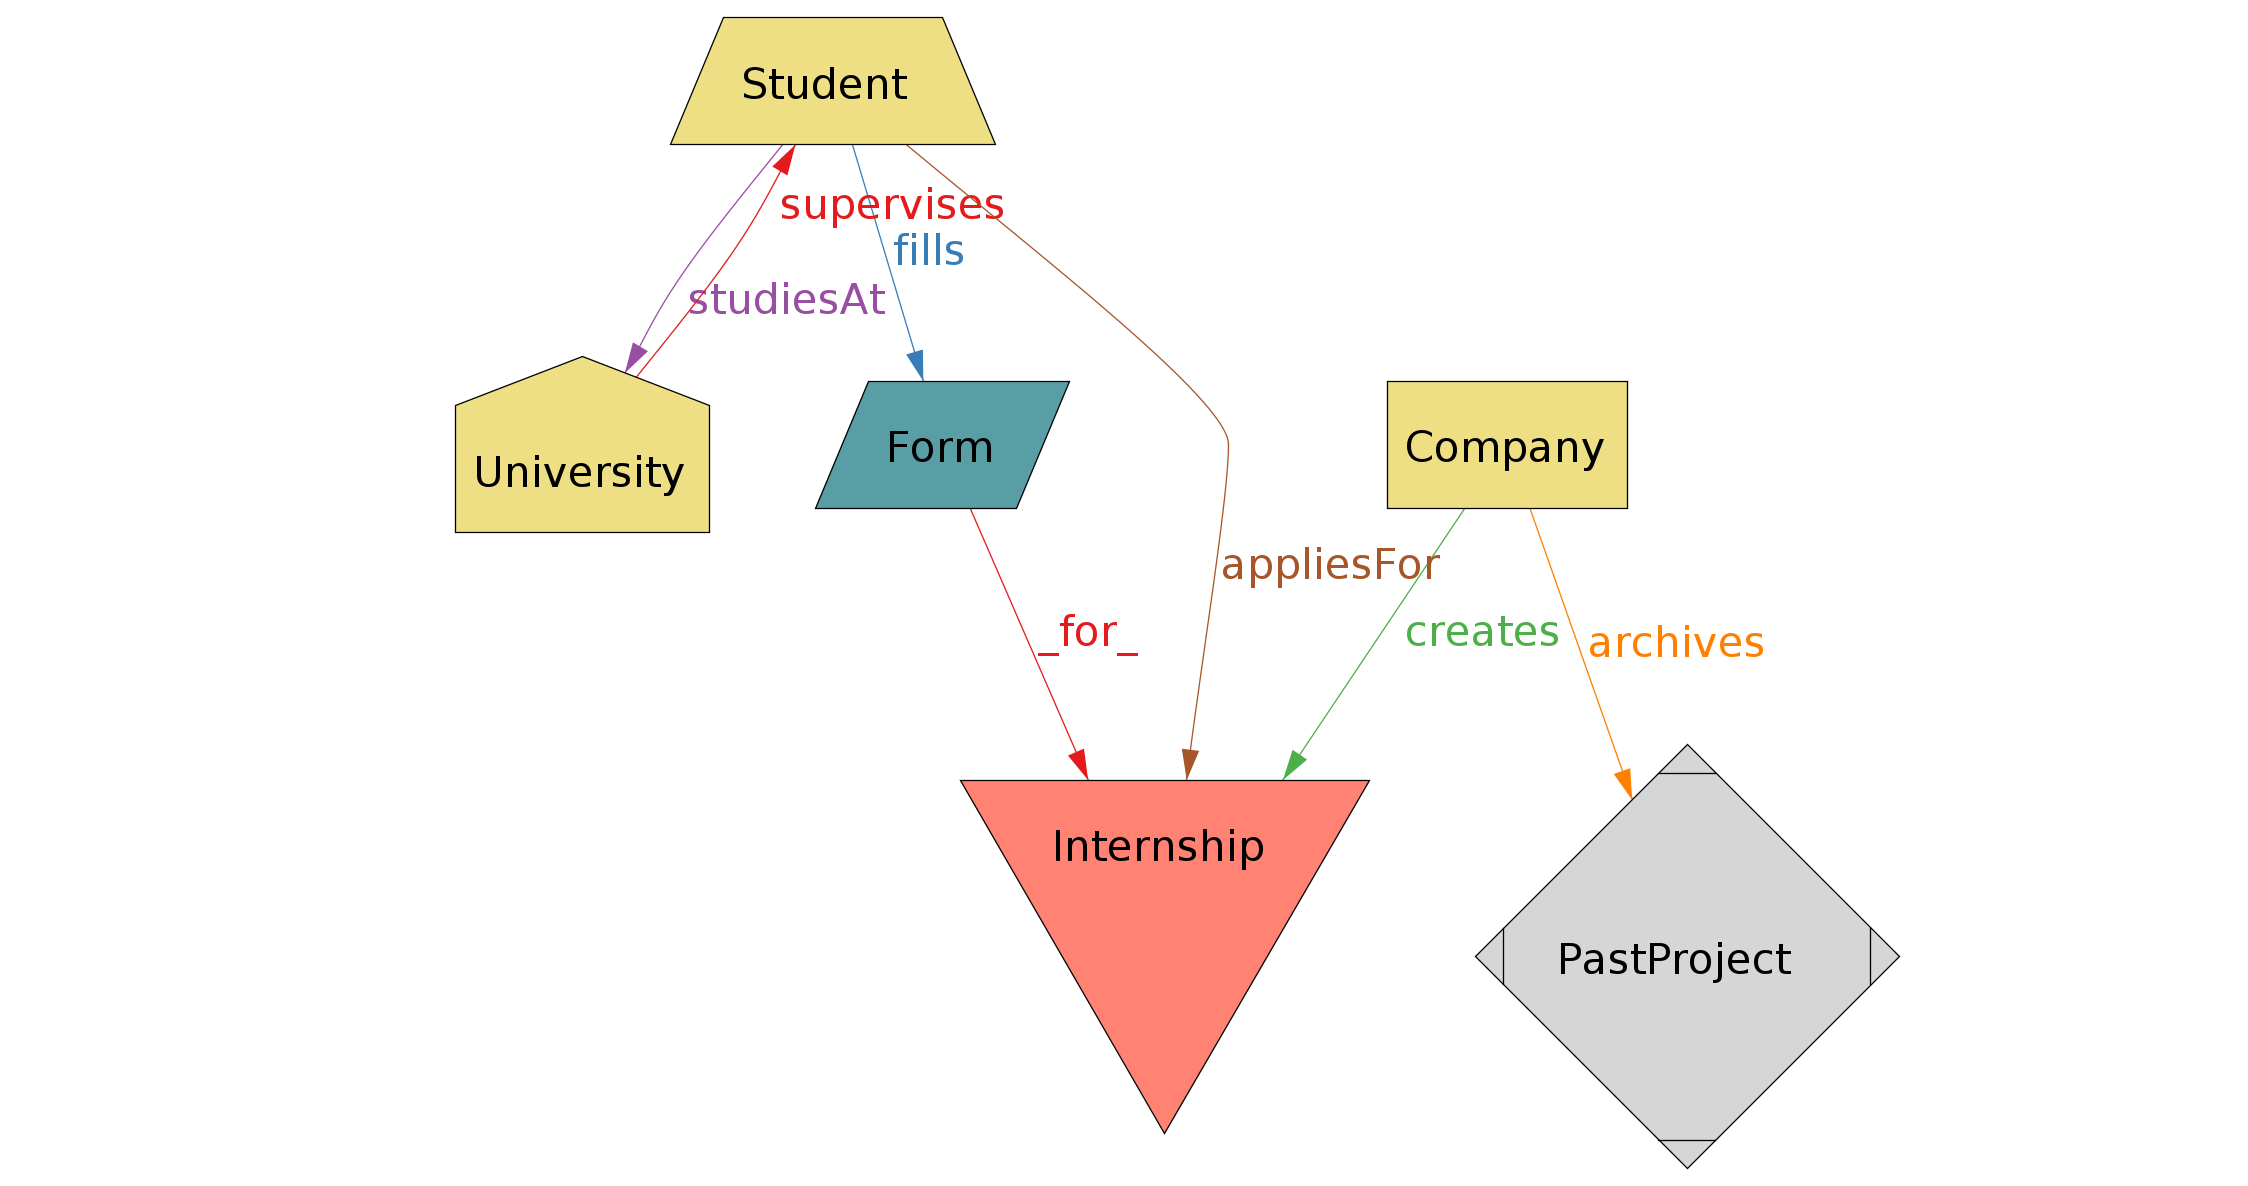
\includegraphics[width=\textwidth]{Images/Scenario1}
\end{center}
We can notice how a company can have an internship already archived as a past project. In addition, we can see how a student that applied can also have filled the form required for the first screening stage of the selection process. \\
\vspace{1\baselineskip} \\
\textbf{Scenario 2:}
{\small
\begin{verbatim}
pred scenarioTwoStudentsCompeting {
    one c: Company, i: Internship | 
    some s1, s2: Student |
        c.creates = i and s1.appliesFor = i and s2.appliesFor = i
        and s1 != s2
}
run scenarioTwoStudentsCompeting for 5 but exactly 1 Company, 1 Internship,
2 Student
\end{verbatim}}
This predicate shows a case where two students apply for the same internship.
\begin{center}
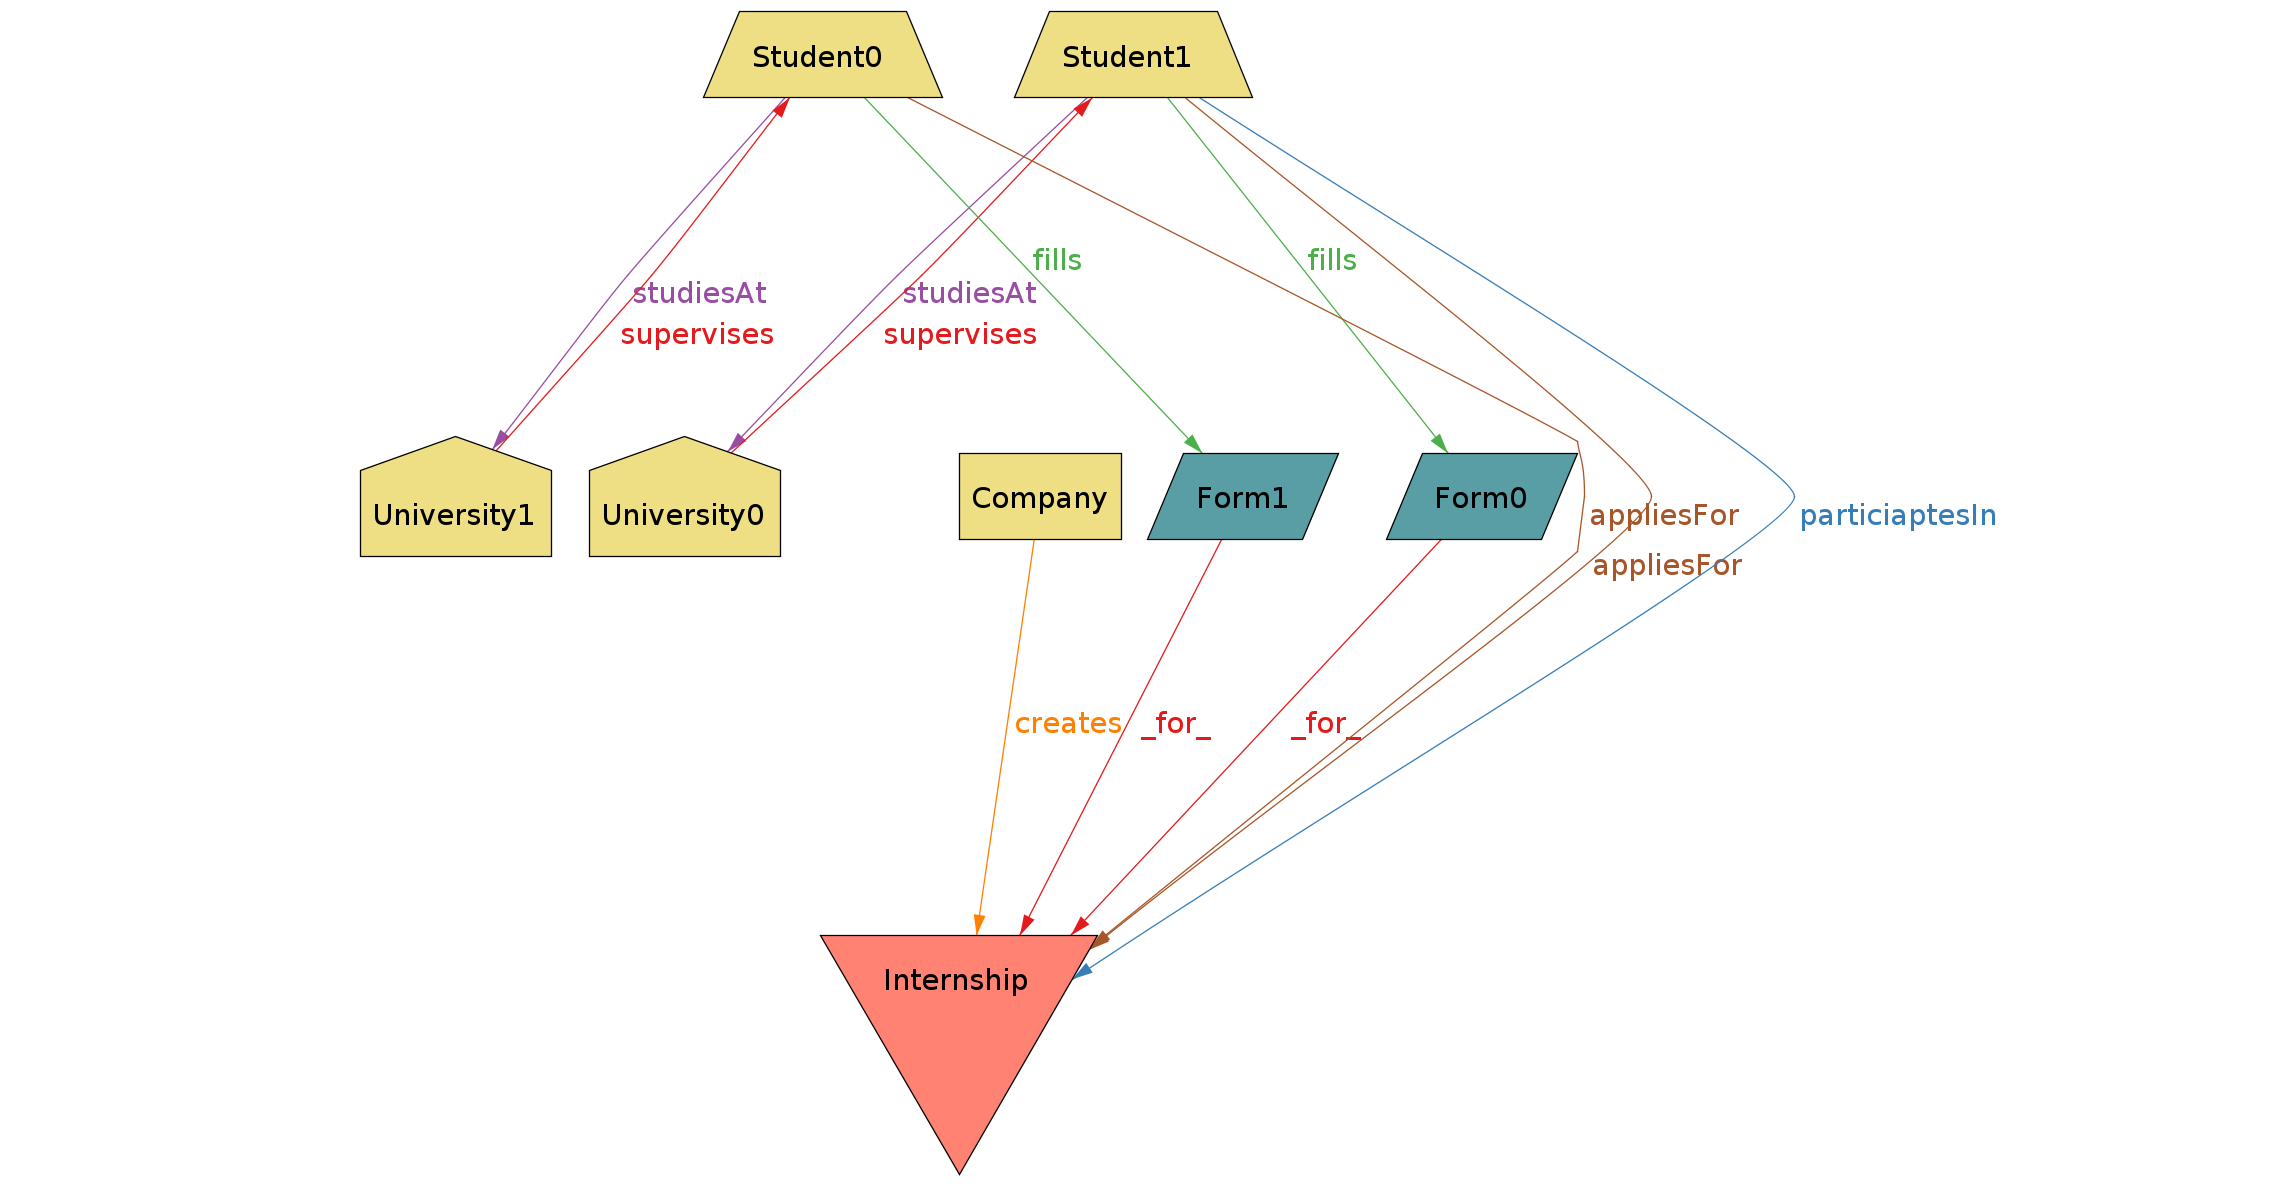
\includegraphics[width=\textwidth]{Images/Scenario2}
\end{center}
\newpage
An important thing to notice is how only one of the candidates actually gets to participate in the internship while the other doesn't get through the final selection. \\
\vspace{1\baselineskip} \\
\textbf{Scenario 3:}
{\small
\begin{verbatim}
pred scenarioMultipleCompaniesMultipleStudents {
    # Company > 2
    # Internship > 2
    # University > 3
    # PastProject < 3
    # Complaint < 4
    one s: Student | #s.appliesFor = 0
    all i: Internship | #i.~appliesFor < 3 and #i.~particiaptesIn < 3
}
run scenarioMultipleCompaniesMultipleStudents for 15 but exactly 7 Student
\end{verbatim}}
\begin{center}
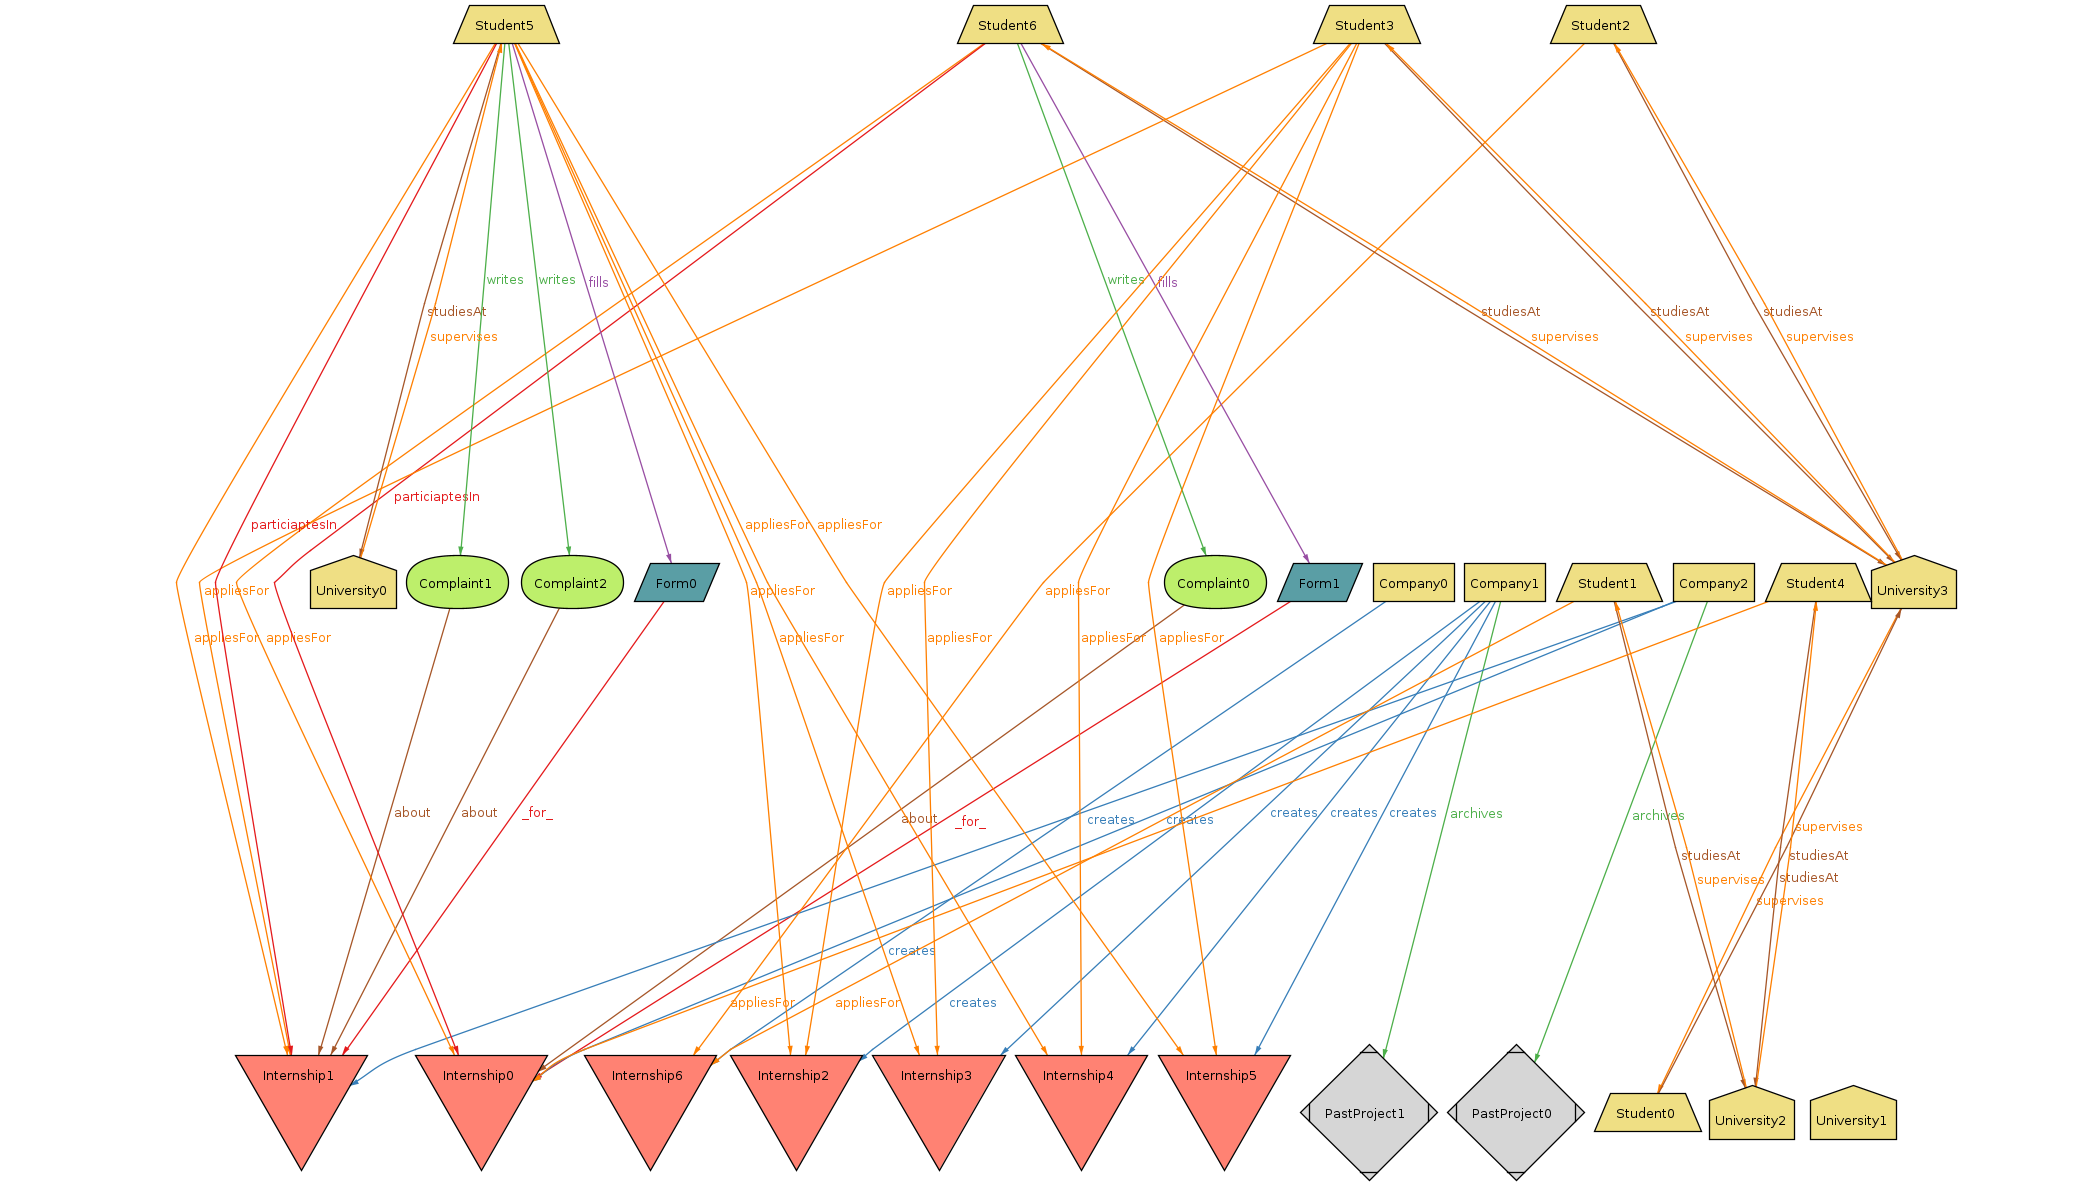
\includegraphics[width=\textwidth]{Images/Scenario3}
\end{center}
This predicate shows almost all cases where we can have students that haven't applied to any internships (student0), universities with no students registered to the platform (university1), companies with some past projects (company1), students that have applied to different internships (student5), students that wrote complaints (student5) and finally candidates participating in internships (student6).

	\subsection{Dynamic model}
This model's purpose is to add a time concept to the system, so that it's possible to model the evolution of its entities and their relations. This will allow us to focus on the dynamic aspects of the possible interactions and use case scenarios of the software-to-be. \\
All of this is made possible thanks to Alloy 6 and the use of time operators like: \textit{var, always, eventually, once, after etc.} to define signatures and constraints that should only be satified under certain conditions.
	\subsubsection{Signatures}
This is a list of all the signatures of the dynamic model, they are quite similar to the ones from the static model, as expected, but some adjustments had to be made to make sure that the new ones reflect the purpose of this model.

{\small
\begin{verbatim}
abstract sig User {}

var abstract sig Report {
    var about: one Internship,
}

sig Student extends User {
	studiesAt: one University,
    var appliesFor: set Internship,
    var participatesIn: set Internship,
    var fills: set Form,
    var writes: set Report,
}

sig Company extends User {
    var creates: set Internship,
    var archives: set Internship,
    var writes: set Report,
}

sig University extends User {
    var supervises: set Student,
    var reads: set Complaint,
}

sig Internship {
    var status: Status
}

var sig Complaint extends Report {}

var sig Feedback extends Report {}

var sig Form {
    var _for_: Internship,
}

enum Status { Open, Screening, Ongoing, Finished, PastProject }

\end{verbatim}
}

	\subsubsection{Facts}
This a list of all the facts which includes all the ones from the static model updated to work with this one and new facts that have to deal with the evolution of the internships, from their creation to their archival.
{\small
\begin{verbatim}
// Facts
// ----------------------------------------------------------------------
// Old facts
// ----------------------------------------------------------------------

// All internships must have exactly one company that offers them or
// has archived them
fact OneOfferingCompany {
    always all i: Internship |
    one c: Company | i in c.creates or i in c.archives
}

// All students must study at exactly one university and that university
// must supervise them
fact EveryStudentBelongsToUniversity {
    always all s: Student | 
    one u: University | (s.studiesAt = u) and (s in u.supervises)
}

// All univesities can only read complaints that are made for internships
// involving their students
fact UniversityReadsRelevantComplaints {
    always all u: University, c: Complaint, i: Internship |
    c.about = i and c in u.reads implies
    once i in u.supervises.participatesIn
}

// Each student can only fill forms for internships that they have applied
// for
fact StudentFillsFormsForAppliedInternships {
    always all s: Student, f: Form |
    f in s.fills implies once f._for_ in s.appliesFor
}

// Each student can submit only one form per internship
fact UniqueFormPerStudentPerInternship {
    always all s: Student, i: Internship |
    lone f: Form | (f in s.fills) and (f._for_ = i)
}

// Each form must be filled by a single student
fact FormFilledBySingleStudent {
    always all f: Form |
    one s: Student | f in s.fills
}

// Each student can only participate in internships for which they have
// applied for and filled a form
fact StudentParticipatesInAppliedInternships {
    always all s: Student, i: Internship |
    i in s.participatesIn implies ((once i in s.appliesFor) and
    (once one f: Form | f._for_ = i and f in s.fills))
}

// A report can only be written by a single student or a single company
// cannot have more than one author
fact UniqueReportAuthor {
    always all r: Report |
    (one s: Student | r in s.writes and no c: Company | r in c.writes) or
    (one c: Company | r in c.writes and no s: Student | r in s.writes)
}

// A report can only be written by a student who is participating/has participated 
// in the internship
fact ReportWrittenByParticipatingStudent {
    always all s: Student, r: s.writes, i: Internship |
    (r.about = i and r in s.writes) implies once i in s.participatesIn
}

// A company can only write reports for an internship it has created and
// in which at least one student participates
fact ReportWrittenByOfferingCompany {
    always all r: Report, c: Company, i: Internship |
    (r.about = i and r in c.writes) implies (r.about in c.creates and
    some s: Student | once r.about in s.participatesIn)
}

// Each student or company can only write one feedback for each internship
// they are involved in
fact UniqueFeedbackPerInternship {
    always all s: Student, c: Company, i: Internship |
    lone f: Feedback | (f in s.writes or f in c.writes) and f.about = i
}

// ----------------------------------------------------------------------
// New facts
// ----------------------------------------------------------------------

// A student can only apply for internships that are open
fact StudentAppliesForOpenInternships {
    always all s: Student, i: Internship |
    i in s.appliesFor implies i.status = Open
}

// A student can only fill forms for internships during the screening phase
fact StudentFillsFormsDuringScreening {
    always all s: Student, f: Form |
    f in s.fills implies f._for_.status = Screening
}

// A student can only participate in internships that are ongoing
fact StudentParticipatesInOngoingInternships {
    always all s: Student, i: Internship |
    i in s.participatesIn implies i.status = Ongoing
}

// A complaint can only be made for internships that are ongoing
fact ComplaintMadeForOngoingInternship {
    always all c: Complaint |
    c.about.status = Ongoing
}

// A feedback can only be written for internships that are finished
fact FeedbackWrittenForFinishedInternship {
    always all f: Feedback |
    f.about.status = Finished
}

// A company can only remove an internship that is finished
fact CompanyCannotRemoveOngoingInternship {
    always all c: Company, i: Internship |
    i in c.creates and i.status != Finished implies i in c.creates'
}

// All internships will eventually be finished
fact AllInternshipsFinish {
    eventually all i: Internship |
    i.status = Finished
}

// All finished internships will eventually be archived by
// the company that created them
fact ArchiveFinishedInternships {
    always all c: Company, i: c.creates |
    i.status = Finished implies after (i.status = PastProject 
    and i in c.archives)
}

// A company can only archive an internship that is a past project
fact CompanyArchivesPastProject {
    always all c: Company, i: c.archives |
    i.status = PastProject
}

// The order of the statuses of an internship must be preserved
fact StatusOrder {
    always all i: Internship |
    (i.status = Open implies i.status' = Screening or i.status' = Open)
    and (i.status = Open implies eventually i.status = Screening)
    and (i.status = Screening implies i.status' = Ongoing)
    and (i.status = Ongoing implies i.status' = Finished)
    and (i.status = Finished implies i.status' = PastProject)
    and (i.status = PastProject implies i.status' = PastProject)
}
\end{verbatim}
}

	\subsubsection{Scenario}
Here we will present a comprehensive scenario that will give us a view of how the model can evolve over time.
{\small
\begin{verbatim}
pred InitialSituation {
    # Student = 3
    # Company = 2
    # University = 2
    # Internship = 3
    all i: Internship |
    i.status = Open
}

pred InternshipApplication {
    always all s: Student, i: Internship |
    i.status = Open implies i in s.appliesFor
}

pred InternshipExecution {
    always all i: Internship |
    (i.status = Ongoing implies some s: Student | i in s.participatesIn) and
    (i.status = Ongoing implies some cl: Complaint | cl.about = i) and
    (i.status = Ongoing implies some cl: Complaint, u: University | cl in u.reads) and
    (i.status = Finished implies some f: Feedback | f.about = i) and
    (i.status = Finished implies some c: Company, s: Student | # c.writes > 0 and 
     # s.writes > 0)
}

pred show {
    InitialSituation;InternshipApplication;
    InternshipExecution
}
run show for 7
\end{verbatim}}
When we run the "show" predicate the Visualizer provides a step-by-step progression of the model's entities and relationships. \\
In this initial step we can see three internships that are open and two students who are applying for them.
\begin{center}
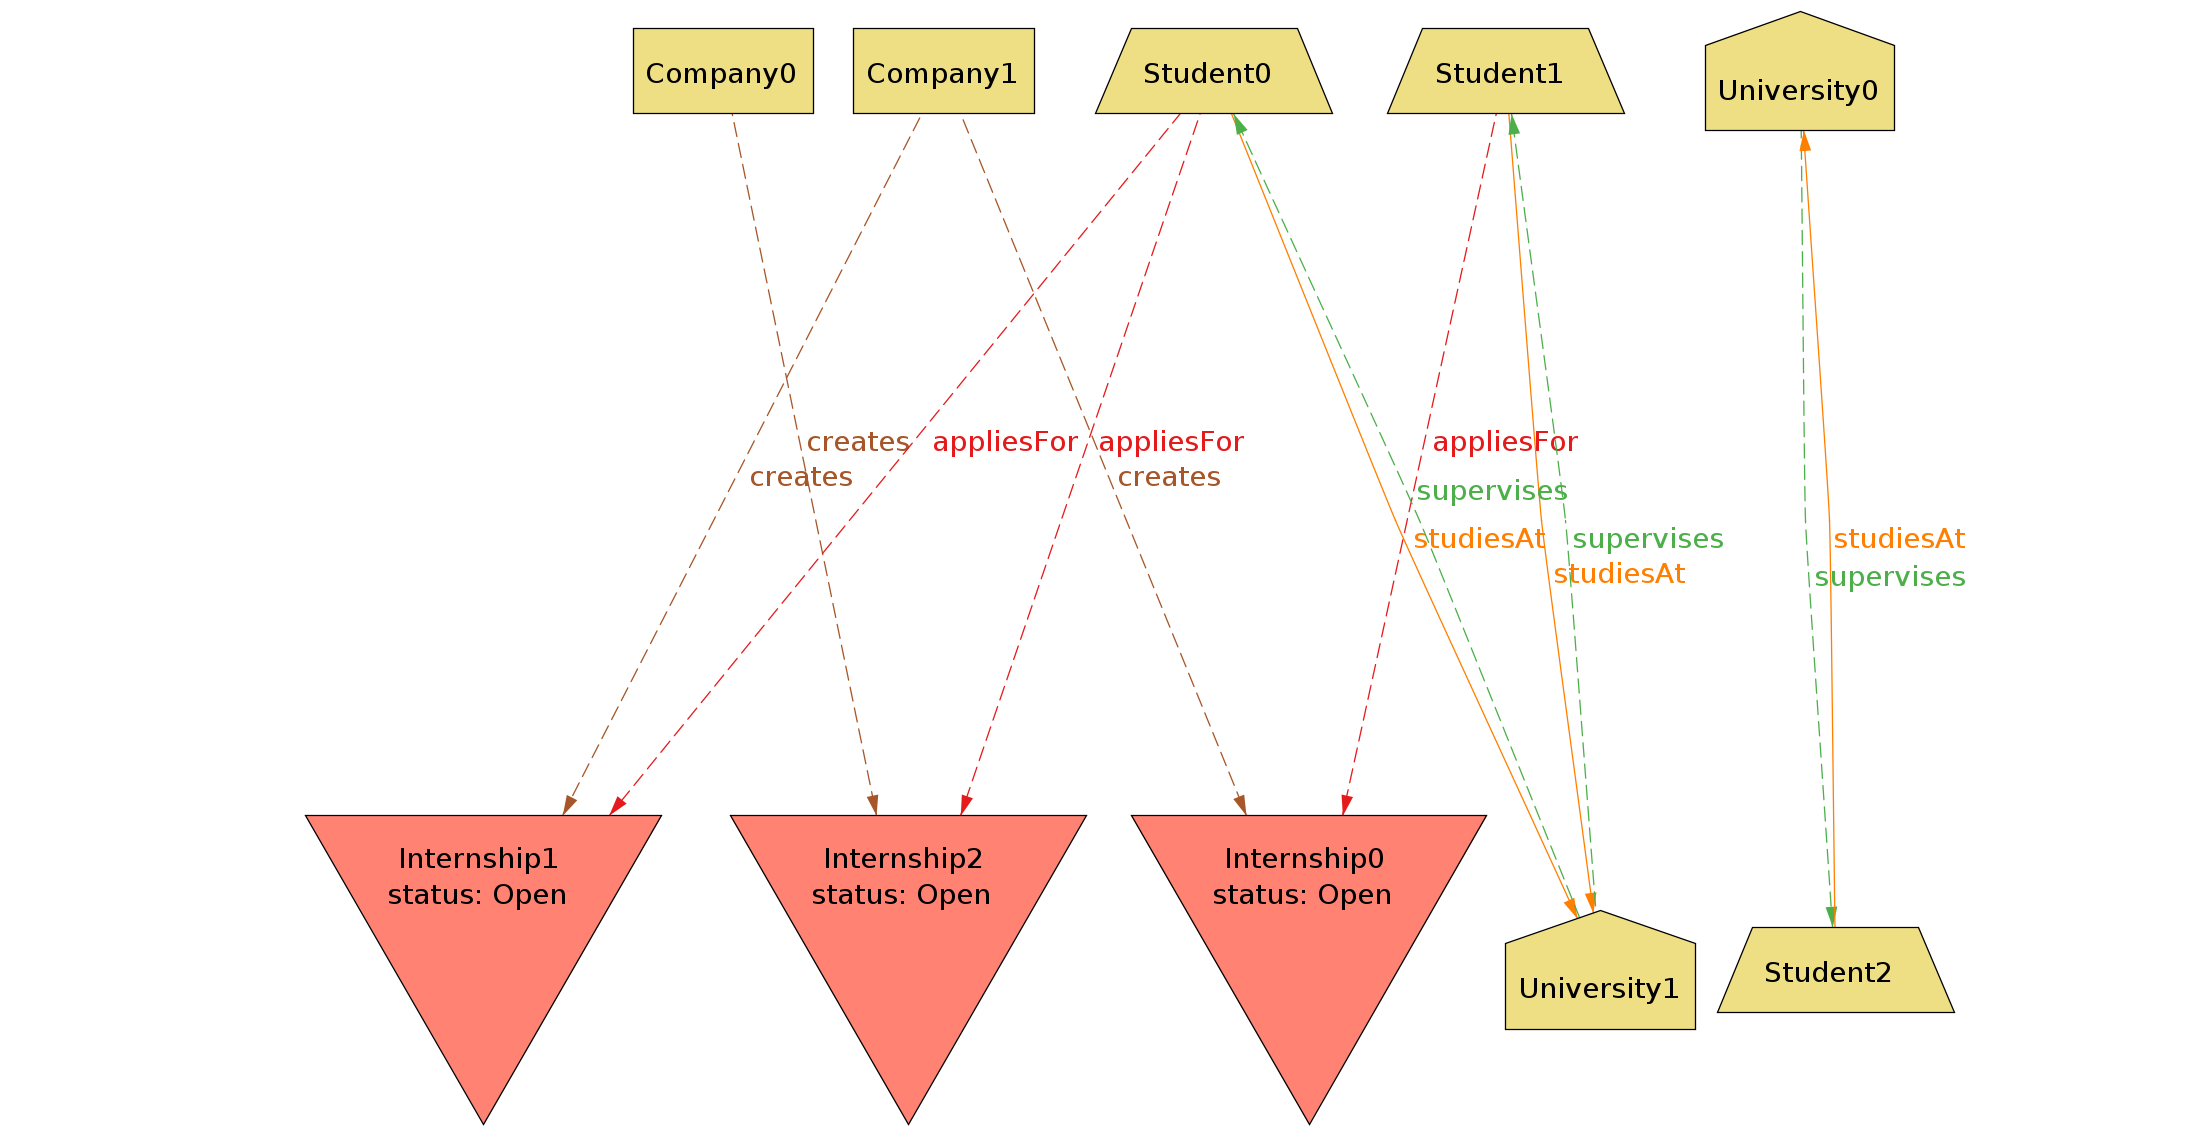
\includegraphics[width=\textwidth]{Images/Scene_step0}
\end{center}
\newpage
Now, we can see that the students who applied have also filled the forms for the screening phase of the internships.
\begin{center}
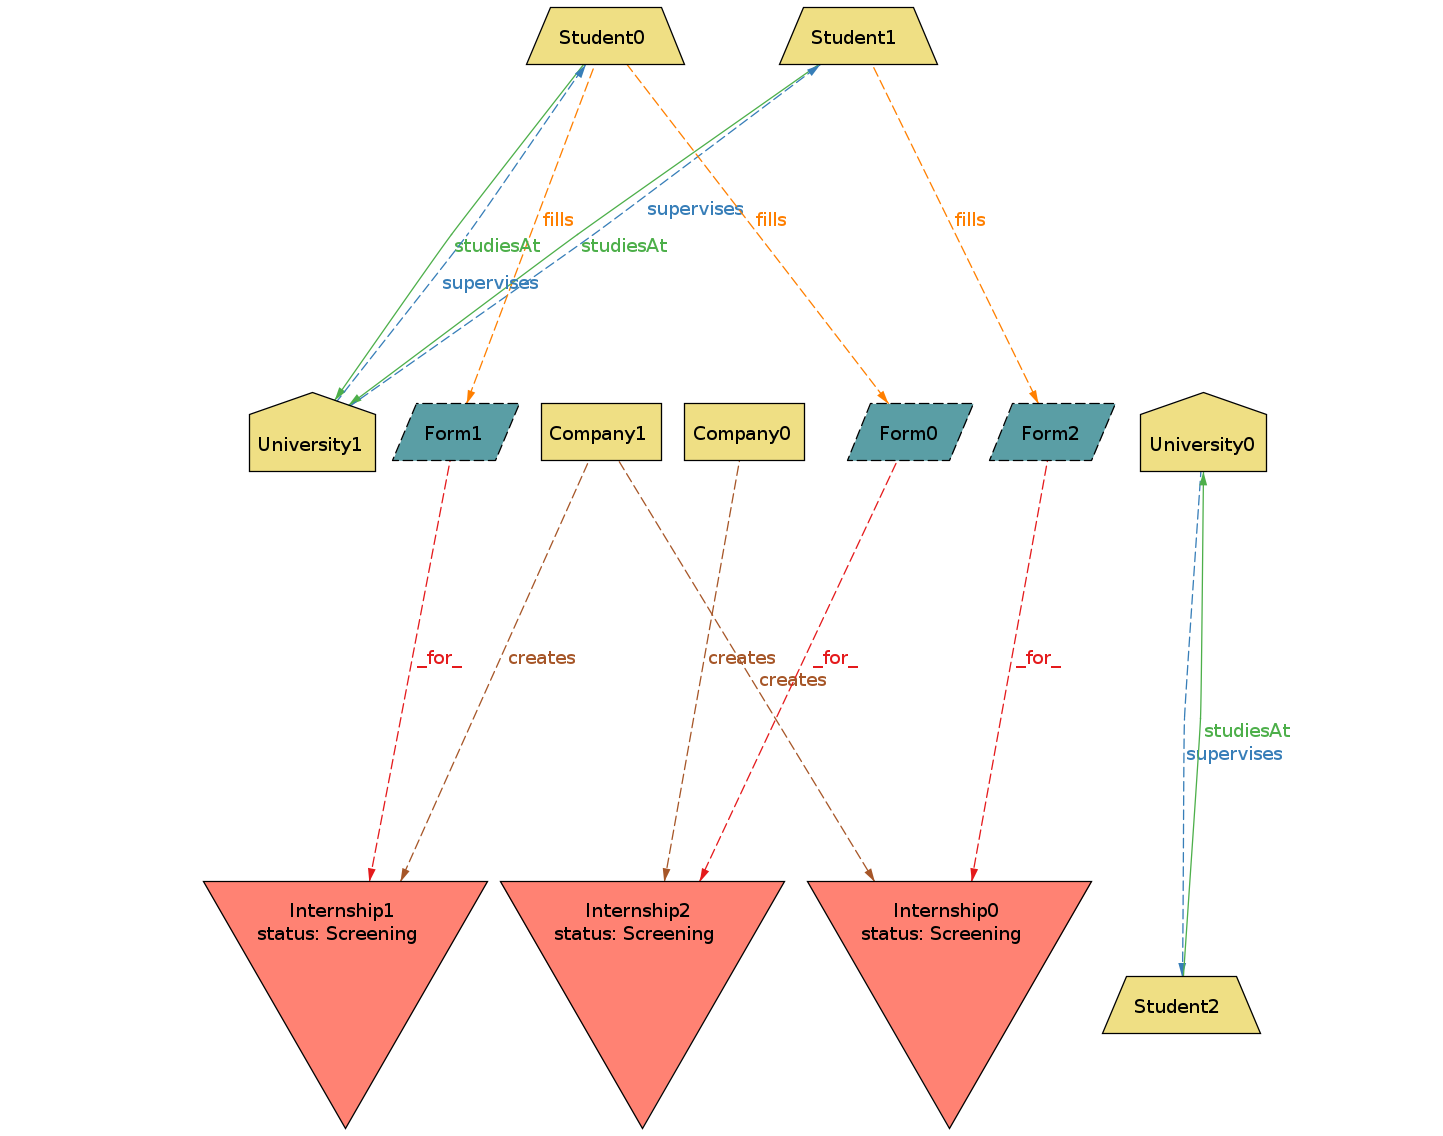
\includegraphics[width=\textwidth]{Images/Scene_step1}
\end{center}
\newpage
At this step, the students are all participating in the internships they have applied for and we can see some complaints written by them regarding those internships and one is read by an involved university. For simplicity's sake, we didn't model the interviews, so we assume that they did them and passed the final screening.
\begin{center}
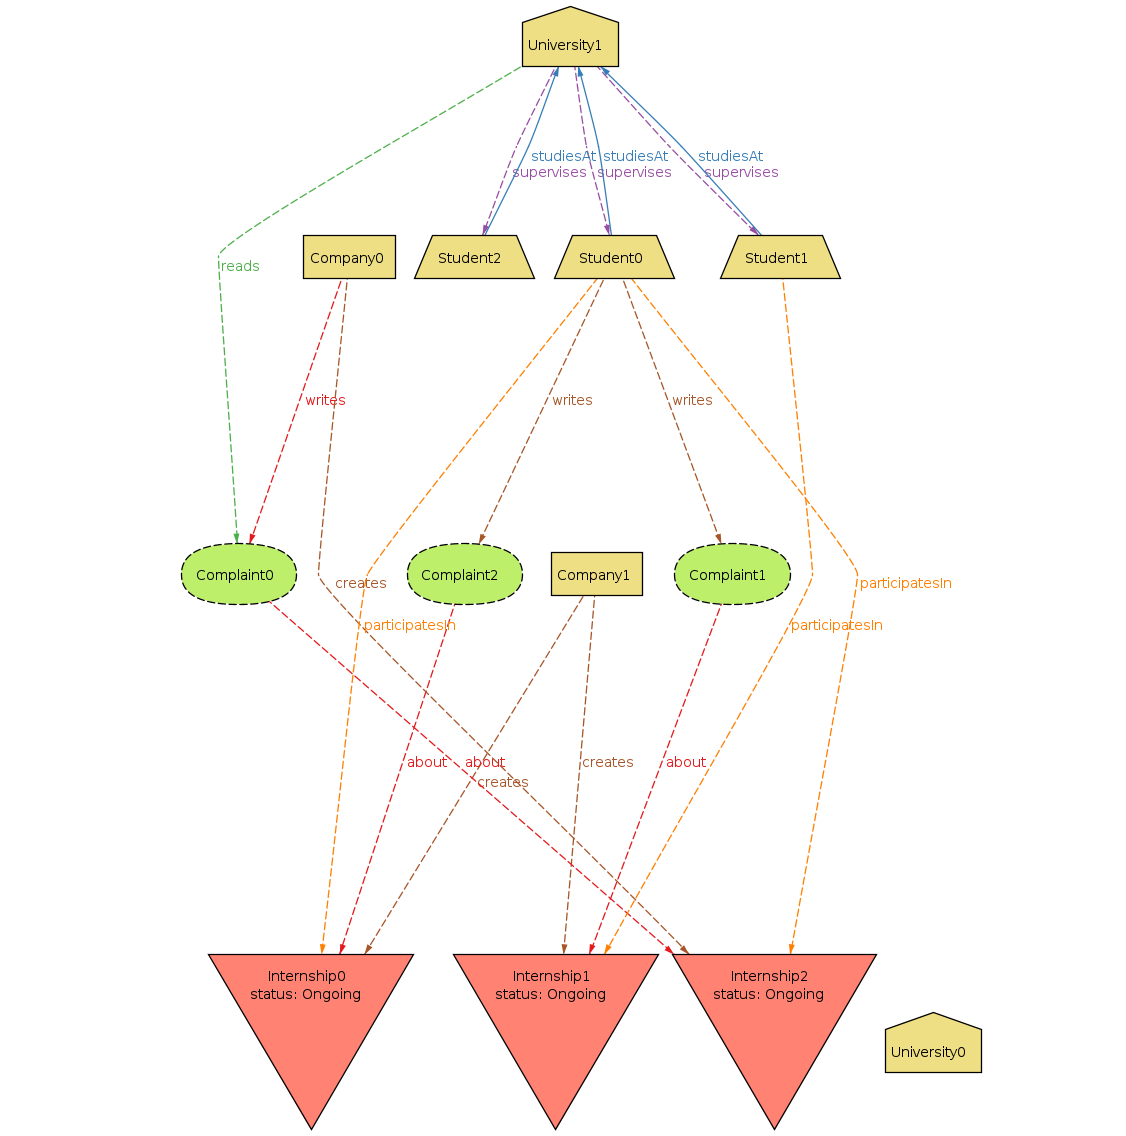
\includegraphics[width=\textwidth]{Images/Scene_step2}
\end{center}
Here, we can see that the internships have concluded and the students have written some feedbacks about them.
\begin{center}
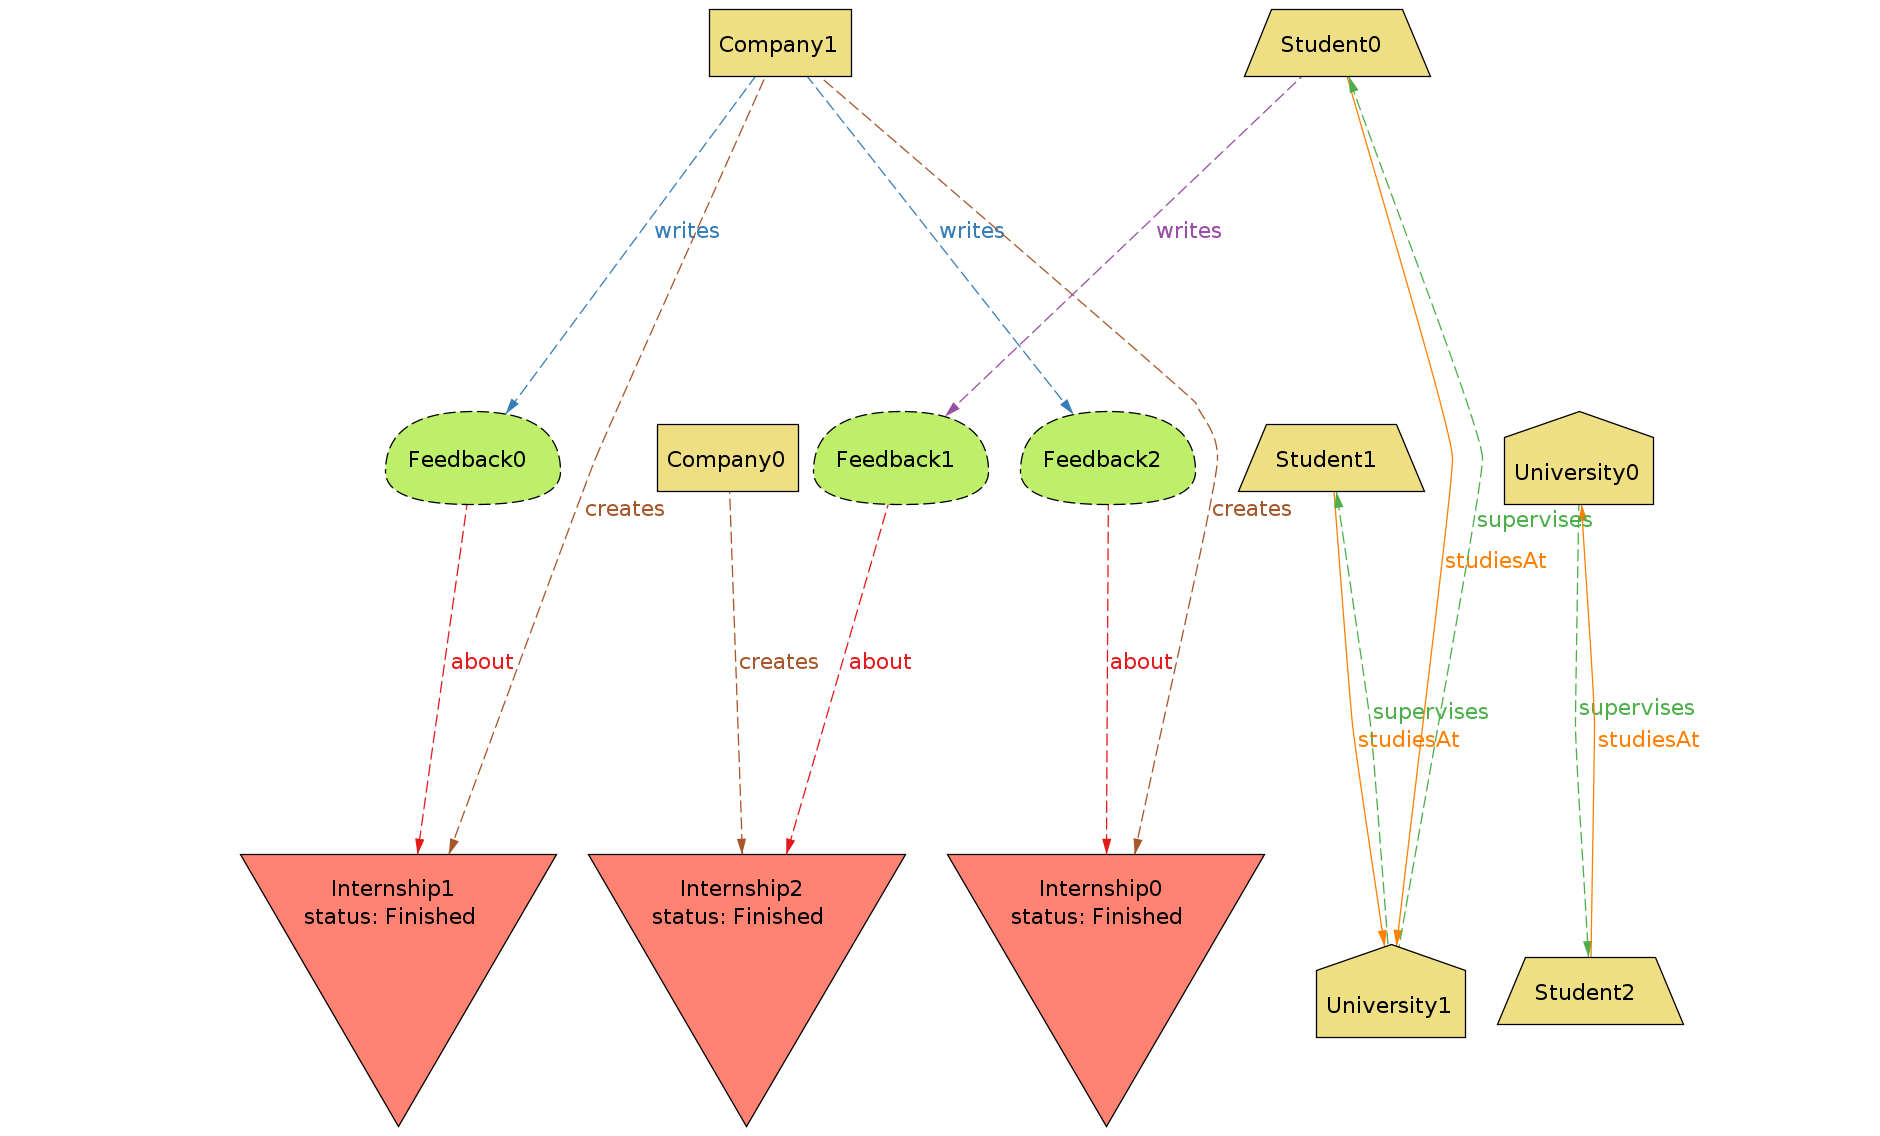
\includegraphics[width=\textwidth]{Images/Scene_step3}
\end{center}
\newpage
Finally, the companies decide to archive the concluded internships transforming them into past projects. Another thing of importance to note is our decision in modeling past projects simply as a state of the internships instead of a new entity like we did in the static model, this was another consequence of the dynamic nature of this model.
\begin{center}
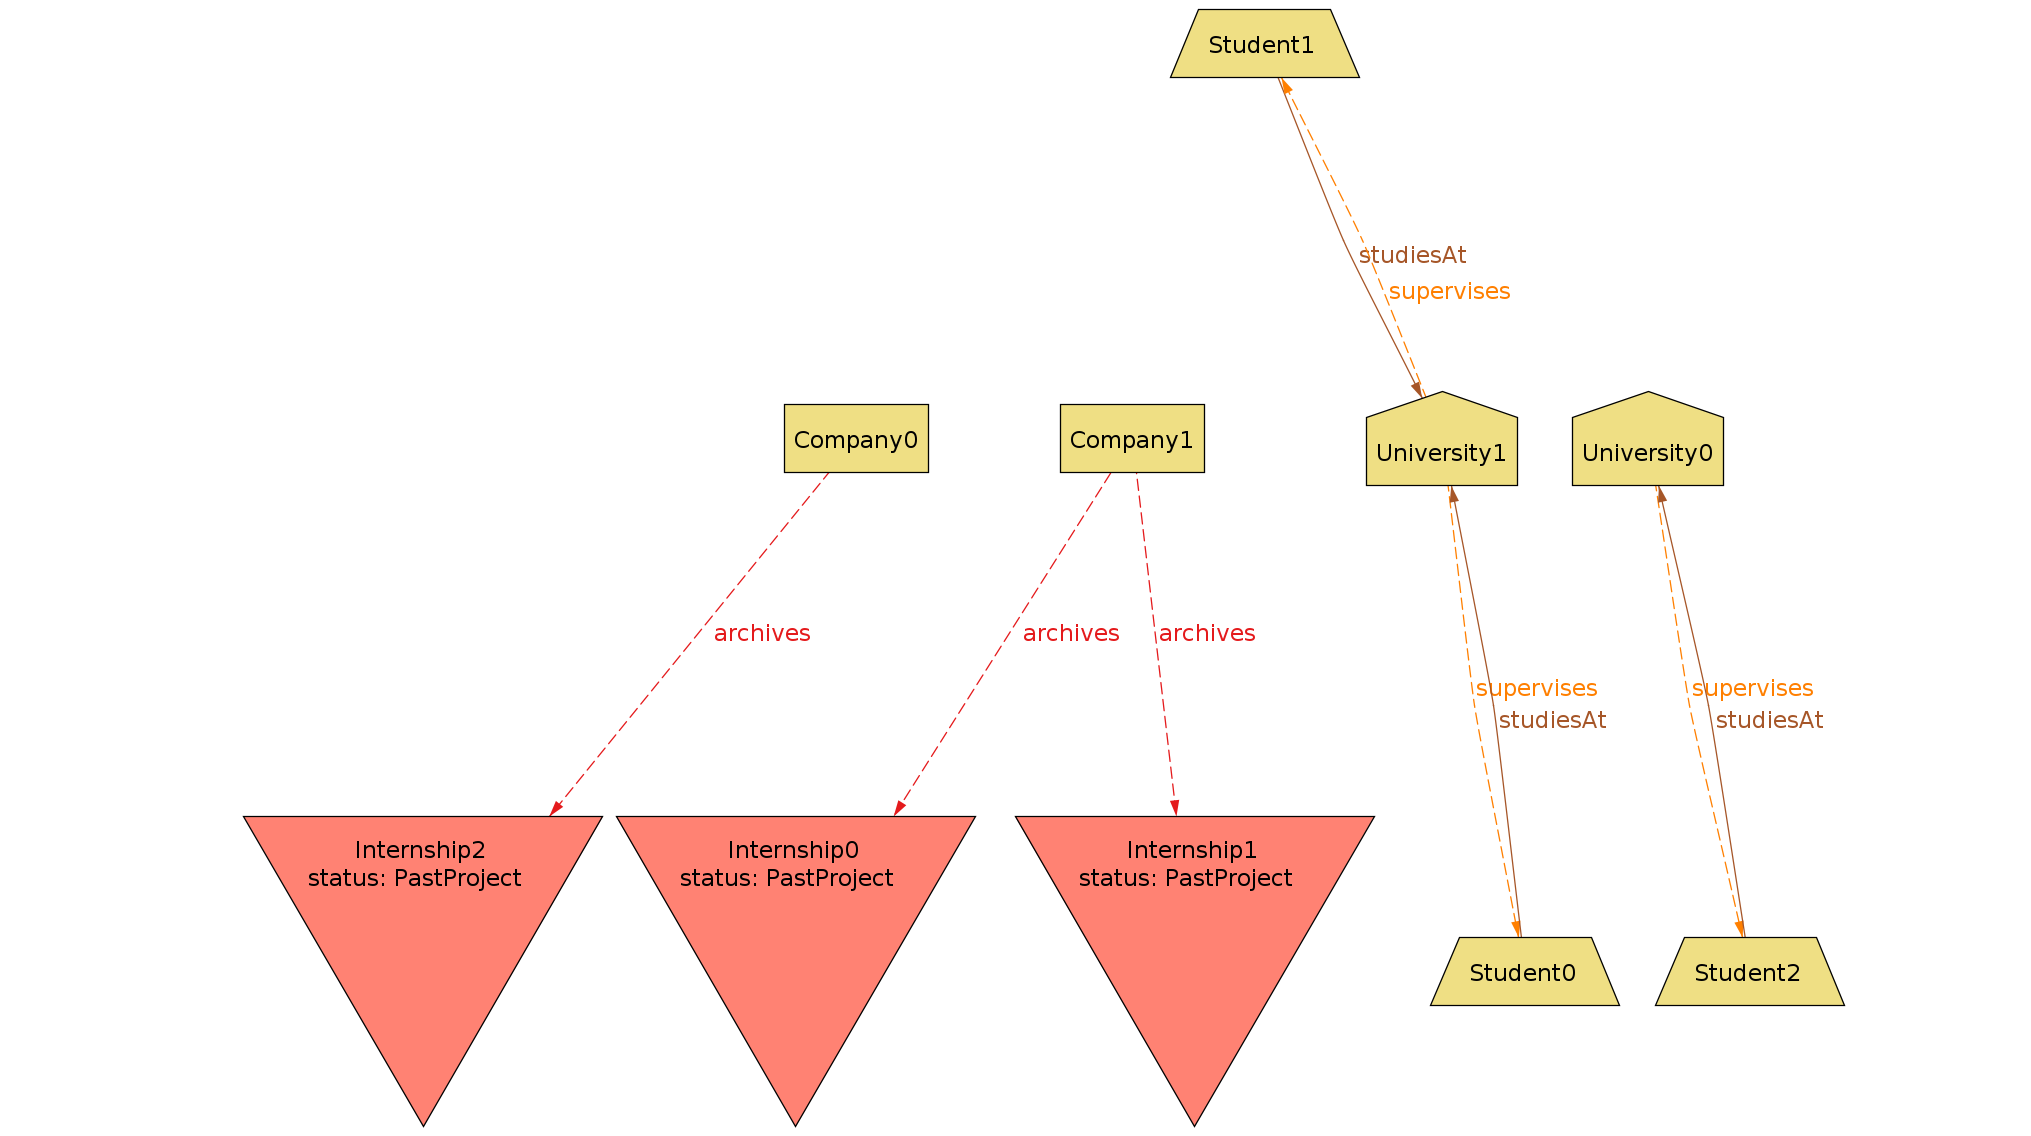
\includegraphics[width=\textwidth]{Images/Scene_step4}
\end{center}
\newpage

\section{Effort spent}
\begin{itemize}

\item \textbf{Abdallah Alkhetiar}
\begin{table}[H]
\begin{tabular}{| >{\centering\arraybackslash}m{0.2\textwidth} || >{\centering\arraybackslash}m{0.2\textwidth} |}
\hline
\textbf{Chapter} & \textbf{Effort} \\
\hline
1 & 10 h \\
\hline
2 & 0 h \\
\hline
3 & 0 h \\
\hline
4 & 0 h \\
\hline
\end{tabular}
\end{table}

\vspace{1\baselineskip}

\item \textbf{Daniel Bonardi}
\begin{table}[H]
\begin{tabular}{| >{\centering\arraybackslash}m{0.2\textwidth} || >{\centering\arraybackslash}m{0.2\textwidth} |}
\hline
\textbf{Chapter} & \textbf{Effort} \\
\hline
1 & 10 h \\
\hline
2 & 0 h \\
\hline
3 & 0 h \\
\hline
4 & 0 h \\
\hline
\end{tabular}
\end{table}

\end{itemize}

\newpage

\section{References}
\textbf{Standard compliance}\\
\href{https://www.enterprisestorageforum.com/management/7-essential-compliance-regulations-for-data-storage-systems/}{\textcolor{blue}{www.enterprisestorageforum.com}}\\
\href{https://beaglesecurity.com/blog/article/software-compliance-standards.html}{\textcolor{blue}{https://beaglesecurity.com}}
\vspace{1\baselineskip} \\
\textbf{Software system attributes}\\
\href{https://testsigma.com/blog/software-quality-attributes/}{\textcolor{blue}{https://testsigma.com}}
\vspace{1\baselineskip} \\
\textbf{Version control}\\
\href{https://github.com/resources/articles/software-development/what-is-version-control}{\textcolor{blue}{https://github.com}}

\end{document}